\documentclass[10pt]{article}

\usepackage[letterpaper,margin=0.8in]{geometry}
\usepackage[T1]{fontenc}
\usepackage{lmodern,microtype,fancyhdr}
\pagestyle{fancy}
\fancyhf{}
\fancyhead[L]{\small EECE5644: Machine Learning and Pattern Recognition}
\fancyhead[R]{\small Assignment 1}
\fancyfoot[C]{\thepage}
\setlength{\headheight}{14pt}
\setlength{\parskip}{3pt}
\setlength{\parindent}{0pt}
\setlength{\emergencystretch}{2em}
\setlength{\textfloatsep}{10pt}
\setlength{\intextsep}{10pt}
\usepackage{amsmath,amssymb,bm}
\usepackage{graphicx,booktabs,float,caption,subcaption}
\usepackage{listings,xcolor}
\usepackage[hidelinks]{hyperref}
\usepackage{enumitem}
\setlist{nosep,leftmargin=*}
\lstset{basicstyle=\ttfamily\scriptsize,breaklines=true,frame=single,columns=fullflexible,numbers=left,numberstyle=\tiny\color{gray},numbersep=7pt,
  keywordstyle=\color{blue!60!black},commentstyle=\color{green!40!black},language=Python,showstringspaces=false}
\captionsetup{font=small}
\newcommand{\x}{\mathbf{x}}
\newcommand{\m}{\mathbf{m}}
\newcommand{\w}{\mathbf{w}}
\newcommand{\tr}{\operatorname{tr}}

\title{EECE5644 Fall 2026 --- Assignment 1}
\author{David Abu}
\date{October 2026}

\begin{document}
\maketitle

\paragraph{Declaration of external resources and AI use.}
Claude (Anthropic) generated the initial implementation and report. OpenAI Codex reviewed and reran the experiments, corrected ROC integration and validation preprocessing, added official-data provenance and numerical checks, and refined this report. The mathematical derivations and code are AI-assisted; the independent reruns and numerical checks are described below. Software: Python, NumPy, SciPy, pandas, Matplotlib, and LaTeX. The experiments reported here use the original UCI Wine Quality and Human Activity Recognition archives; exact download URLs and SHA-256 hashes are included below. The instructor's assignment permits AI assistance when it is acknowledged.

\paragraph{Notation and loss convention.} $\lambda_{ij}$ is the loss for deciding $D=i$ when the true label is $L=j$. All random data are generated once with fixed seeds, saved to disk, and the same data are used for every part of a question.

%==========================================================================
\section*{Question 1: Gaussian classifiers and Fisher LDA}

Generated $N=10{,}000$ samples ($L=1$ with probability 0.65): $N_0=3460$, $N_1=6540$. Seed 5644; data saved in \texttt{q1\_data.npz}.

\subsection*{Part A: ERM with the true pdf}

\textbf{1. Decision rule.} The conditional risk of decision $i$ is $R(D{=}i\mid\x)=\sum_j\lambda_{ij}P(L{=}j\mid\x)$. Deciding $D=1$ is optimal iff $R(D{=}1|\x)<R(D{=}0|\x)$:
\begin{gather*}
\lambda_{10}P(L{=}0|\x)+\lambda_{11}P(L{=}1|\x) < \lambda_{00}P(L{=}0|\x)+\lambda_{01}P(L{=}1|\x)\\
\iff (\lambda_{01}-\lambda_{11})\,p(\x|L{=}1)P(L{=}1) > (\lambda_{10}-\lambda_{00})\,p(\x|L{=}0)P(L{=}0),
\end{gather*}
using Bayes' rule and cancelling $p(\x)$. Assuming $\lambda_{01}>\lambda_{11}$, the minimum-expected-risk rule is the likelihood-ratio test
\[
\boxed{\;\frac{p(\x\mid L=1)}{p(\x\mid L=0)} \;\underset{D=0}{\overset{D=1}{\gtrless}}\; \gamma=\frac{(\lambda_{10}-\lambda_{00})\,P(L=0)}{(\lambda_{01}-\lambda_{11})\,P(L=1)}\;}
\]
For arbitrary nonnegative losses, the undivided inequality above remains valid. If $\lambda_{01}-\lambda_{11}<0$, division reverses the inequality; if it is zero, compare the remaining term directly. Equal conditional risks may be resolved by a fixed tie convention.

For minimum probability of error (0--1 loss: $\lambda_{00}=\lambda_{11}=0$, $\lambda_{01}=\lambda_{10}=1$): $\gamma^*=P(L{=}0)/P(L{=}1)=0.35/0.65=0.5385$, $\ln\gamma^*=-0.619$.
With Gaussian class conditionals the test is implemented in the log domain (numerically stable, monotone so equivalent):
\[
\ln\frac{p(\x|1)}{p(\x|0)} = -\tfrac12(\x-\m_1)^T C_1^{-1}(\x-\m_1)+\tfrac12(\x-\m_0)^T C_0^{-1}(\x-\m_0)-\tfrac12\ln\frac{|C_1|}{|C_0|}\;\gtrless\;\ln\gamma .
\]
This is a quadratic discriminant, since $C_0\neq C_1$.

\textbf{2. ROC.} The score $s(\x_n)=\ln[p(\x_n|1)/p(\x_n|0)]$ was computed for all samples. Sweeping $\ln\gamma$ from $-\infty$ through every observed score value (10{,}001 thresholds) gives every distinct operating point the data can produce; for each, $P(D{=}1|L{=}1;\gamma)$ and $P(D{=}1|L{=}0;\gamma)$ are estimated by counts. At $\gamma=0$ the curve is at $(1,1)$; at $\ln\gamma=\max_n s(\x_n)$ (finite) it reaches $(0,0)$. Both $P(D{=}1|L{=}0;\gamma)$ and $P(D{=}0|L{=}1;\gamma)=1-P(D{=}1|L{=}1;\gamma)$ are stored for each threshold.

\textbf{3. Minimum-$P(\text{error})$ threshold.} For each threshold,
\[P(\text{error};\gamma)=P(D{=}1|L{=}0;\gamma)P(L{=}0)+P(D{=}0|L{=}1;\gamma)P(L{=}1);\]
the minimizer is marked on the ROC (Fig.~\ref{fig:q1a}). Any $\gamma$ between two consecutive sorted scores gives the same decisions; I report the midpoint. Results are in Table~\ref{tab:q1}.

\begin{table}[H]\centering\small
\resizebox{\linewidth}{!}{\begin{tabular}{lccccc}
\toprule
Classifier & threshold at min $P(e)$ & $P(D{=}1|L{=}1)$ & $P(D{=}1|L{=}0)$ & $\hat P(\text{error})$ & AUC \\
\midrule
A: true pdf & $\hat\gamma = 0.791$ ($\ln\hat\gamma=-0.235$) & 0.9679 & 0.0145 & 0.0259 & 0.9959 \\
\quad at theory $\gamma^*=0.5385$ & $\ln\gamma^*=-0.619$ & 0.9716 & 0.0225 & 0.0264 & \\
B: naive Bayes & $\hat\gamma = 0.640$ ($\ln\hat\gamma=-0.447$) & 0.9654 & 0.0286 & 0.0325 & 0.9942 \\
\quad at $\gamma^*=0.5385$ & $\ln\gamma^*=-0.619$ & 0.9670 & 0.0318 & 0.0326 & \\
C: Fisher LDA & $\hat\tau = -0.0053$ & 0.9512 & 0.0584 & 0.0521 & 0.9854 \\
\bottomrule
\end{tabular}
}
\caption{Question 1 summary. Probabilities are sample-count estimates on the same 10K samples.}\label{tab:q1}
\end{table}

\begin{figure}[H]\centering
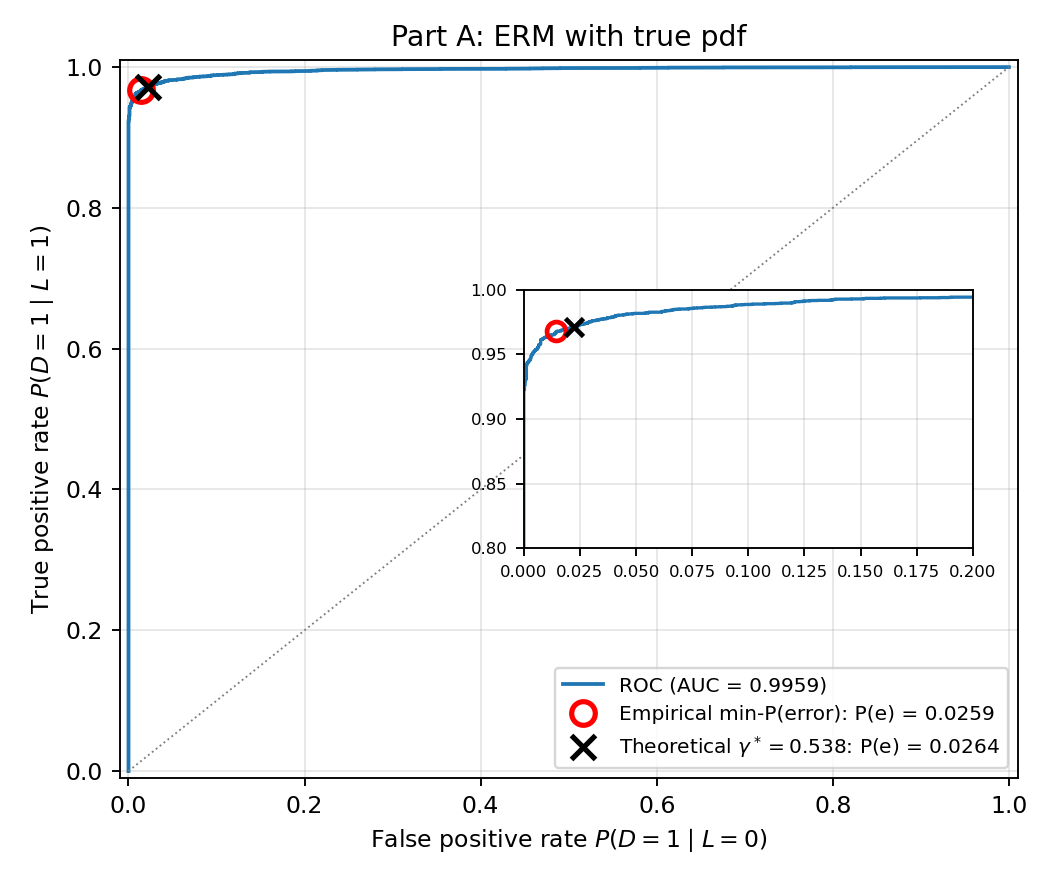
\includegraphics[width=0.49\linewidth]{figs/q1a_roc.png}\hfill
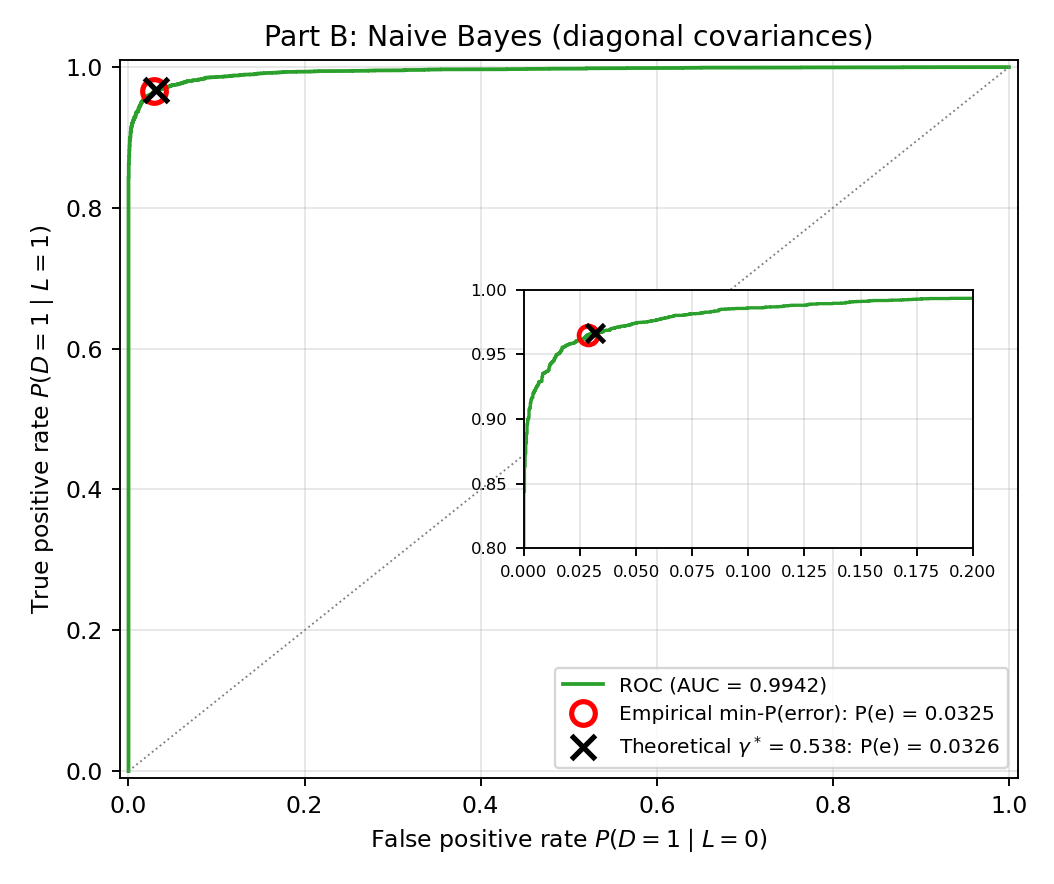
\includegraphics[width=0.49\linewidth]{figs/q1b_roc.png}
\caption{ROC curves of the ERM classifier with the true pdf (left) and the naive Bayes classifier (right). Red circle: empirically selected minimum-$P(\text{error})$ operating point; black cross: operating point at the theoretical threshold $\gamma^*=0.5385$. Insets zoom into the upper-left corner.}\label{fig:q1a}
\end{figure}

\textbf{Estimated minimum $P(\text{error})$} $\approx \mathbf{0.0259}$ (at $\hat\gamma\approx0.79$), versus $0.0264$ at the theoretical $\gamma^*=0.538$. As an independent reference, I evaluated the theoretical rule on a separate 2-million-sample Monte Carlo set: $P(\text{error};\gamma^*)\approx0.0262$, with binomial Monte Carlo standard error approximately $0.000113$ (an approximate 95\% interval is $0.0262235\pm0.0002215$). This estimates the Bayes error; it is not an exact analytic value.

\textbf{Comparison of empirical vs.\ theoretical $\gamma$.} The empirical minimizer ($\hat\gamma\in[0.783,0.799)$) is larger than $\gamma^*=0.538$, yet the two error values differ by only $0.00045$ (about 4--5 of 10{,}000 samples). Figure~\ref{fig:q1perr} shows why: $P(\text{error};\gamma)$ is very flat around its minimum, so with a finite sample the location of the minimum is noisy. The empirical $\hat\gamma$ is fitted to these particular 10K samples, so its error $0.0259$ is optimistically biased (below the large-sample Bayes error $0.0262$). The theoretically derived $\gamma^*$ is the one that is optimal for the distribution; the empirical one only agrees with it up to sampling noise, and would converge to it as $N\to\infty$.

\begin{figure}[H]\centering
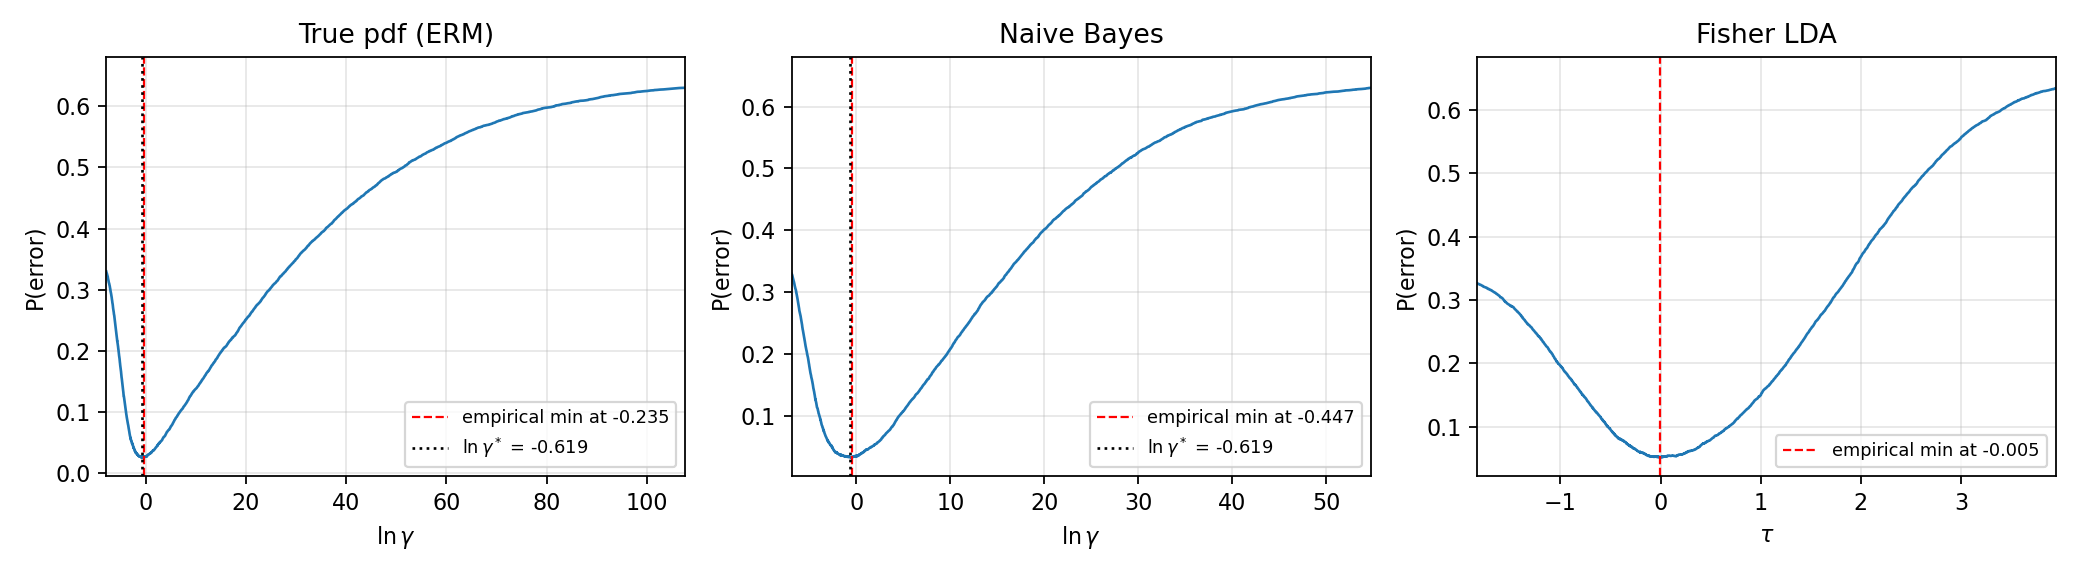
\includegraphics[width=\linewidth]{figs/q1_perr_vs_thr.png}
\caption{Estimated $P(\text{error})$ versus threshold for the three classifiers. Red dashed: empirical minimizer; black dotted: $\ln\gamma^*$.}\label{fig:q1perr}
\end{figure}

\subsection*{Part B: Naive Bayes (diagonal covariance) model mismatch}
The classifier uses the same LRT and threshold formula but with $C_0^{NB}=\operatorname{diag}(C_0)=\operatorname{diag}(0.5,0.25,0.25,0.5)$ and $C_1^{NB}=\operatorname{diag}(C_1)=\operatorname{diag}(1,2,1,3)$, i.e.\ it ignores the correlations among $x_1,x_2,x_3$ ($x_4$ is already uncorrelated). The score is $\ln g(\x|\m_1,C_1^{NB})-\ln g(\x|\m_0,C_0^{NB})$ and the same sweep is performed on the same 10K samples (Fig.~\ref{fig:q1a} right, Table~\ref{tab:q1}).

\begin{itemize}
\item Minimum $\hat P(\text{error}) = \mathbf{0.0325}$ at $\hat\gamma\approx0.640$ (vs.\ $0.0326$ at $\gamma^*=0.538$). Monte Carlo with 2M samples at $\gamma^*$: $0.0322$.
\item The ROC moves down/right (AUC $0.9959\to0.9942$) and the best achievable error rises by about 25\% relative ($0.0259\to0.0325$; $0.0262\to0.0322$ with 2M samples).
\item Here $\gamma^*$ from priors and losses is no longer guaranteed optimal, because the NB ratio is not the true likelihood ratio, so thresholding it at $\gamma^*$ is not the Bayes rule. Empirically the best threshold ($0.64$) is still close to $\gamma^*$ and the error at $\gamma^*$ is almost the same as the minimum.
\end{itemize}
\textbf{Conclusion:} yes, the mismatch hurts, but moderately. The decision boundary is still quadratic and uses the correct means and variances; it changes the shape and orientation of the quadratic discriminant in the $(x_1,x_2,x_3)$ subspace. The correlations ($|\rho|\le 0.5$) are moderate and the class means are well separated (distance 3), so the loss is noticeable but not dramatic.

\subsection*{Part C: Fisher LDA}
Sample-average estimates from the 10K samples:
\[\hat{\m}_0=(-0.500,-0.505,-0.496,-0.498)^T,\quad \hat{\m}_1=(1.011,1.016,0.995,0.983)^T,\]
and
\[\hat C_j=\tfrac1{N_j}\textstyle\sum_{n:L_n=j}(\x_n-\hat\m_j)(\x_n-\hat\m_j)^T\]
(both close to the true $C_0,C_1$).
With equal weights, $S_B=(\hat\m_1-\hat\m_0)(\hat\m_1-\hat\m_0)^T$ and $S_W=\hat C_0+\hat C_1$. The Fisher criterion $J(\w)=\frac{\w^TS_B\w}{\w^TS_W\w}$ is maximized by the generalized eigenvector $S_B\w=\lambda S_W\w$ with the largest eigenvalue ($\lambda_{\max}=4.689$; $S_B$ has rank 1 so this is the only nonzero one). Normalized and oriented so that class 1 projects higher,
\[
\w_{LDA}=(0.6028,\;0.2747,\;0.7086,\;0.2432)^T,
\]
which equals the closed form $S_W^{-1}(\hat\m_1-\hat\m_0)/\|\cdot\|$ (checked numerically). The rule is $D=1$ iff $\w_{LDA}^T\x>\tau$; sweeping $\tau$ over $(-\infty,\infty)$ (all projected values) gives the ROC in Fig.~\ref{fig:q1c}. The error at each $\tau$ is estimated by sample counts, $\#\{\text{errors}\}/N$.

Minimum $\hat P(\text{error})=\mathbf{0.0521}$ at $\hat\tau\approx-0.0053$ ($P(D{=}1|L{=}1)=0.951$, $P(D{=}1|L{=}0)=0.058$), AUC $=0.9854$.

\begin{figure}[H]\centering
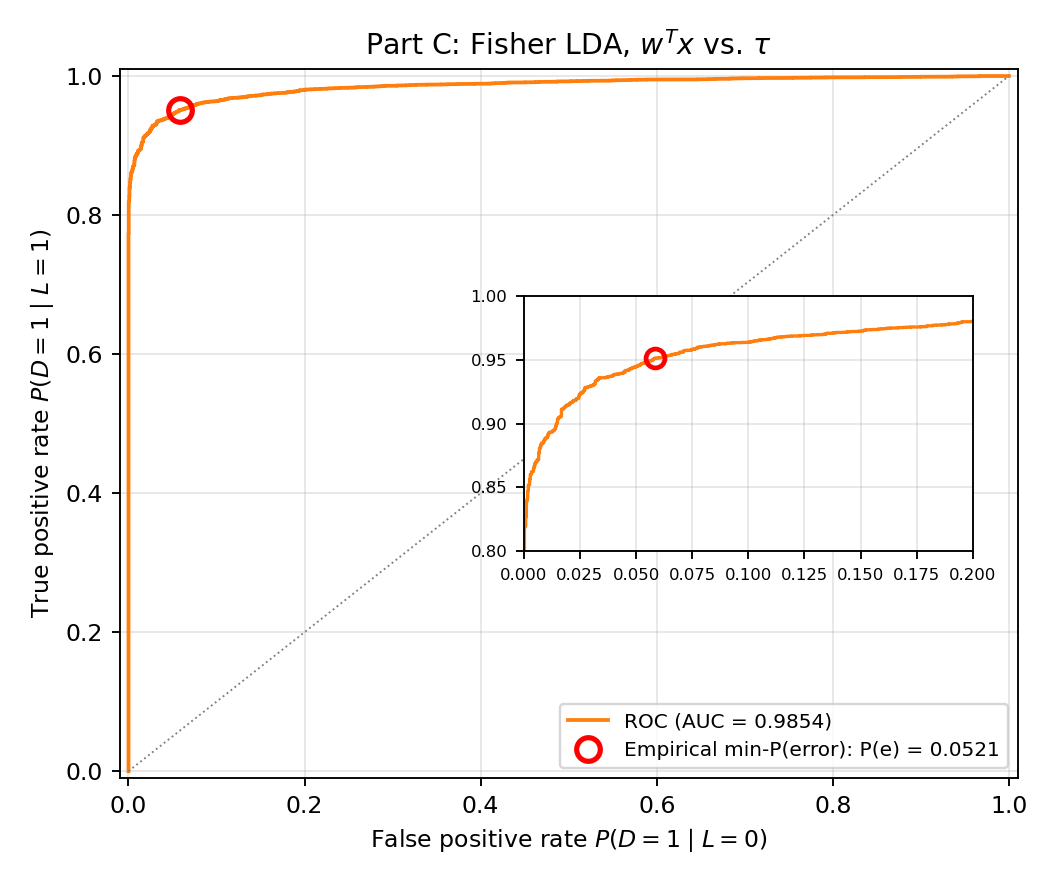
\includegraphics[width=0.49\linewidth]{figs/q1c_roc.png}\hfill
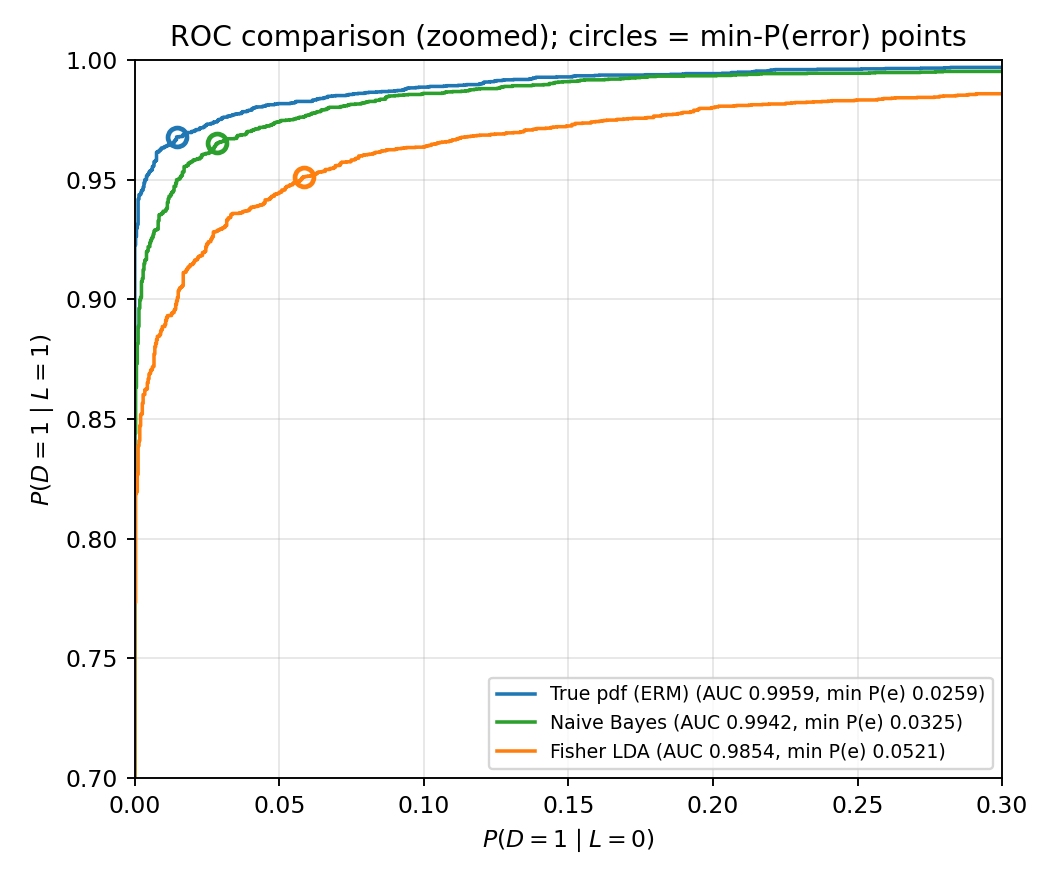
\includegraphics[width=0.49\linewidth]{figs/q1_compare.png}
\caption{Left: Fisher LDA ROC with the minimum-$P(\text{error})$ point. Right: zoomed comparison of the three ROC curves.}\label{fig:q1c}
\end{figure}

\textbf{Discussion.} The ranking is true-pdf ERM ($0.0259$) $<$ naive Bayes ($0.0325$) $<$ LDA ($0.0521$), and the observed ROC curves show the same broad ordering (Fig.~\ref{fig:q1c} right). LDA roughly doubles the error of the optimal classifier. The reason is structural: the Bayes rule is quadratic because $C_1$ has much larger variances than $C_0$ (e.g.\ $\operatorname{var}(x_4)$ is 3 vs.\ 0.5), so the optimal boundary is a closed-ish surface wrapped around the tight class-0 cloud. LDA can only use a hyperplane, and Fisher's criterion maximizes projected mean separation relative to within-class spread; it does not generally minimize error. Under equal-covariance Gaussian models, the Fisher direction agrees with the Bayes linear discriminant when paired with the appropriate threshold. Naive Bayes, although its covariances are wrong, still exploits the covariance difference through a quadratic boundary, which is why it beats LDA here. As instructed, the LDA direction uses equal class weights; the unequal class frequencies still enter the sample-count error used to choose $\tau$. LDA's advantages are that it needs no distributional knowledge and only $d$ projection parameters.

%==========================================================================
\clearpage\section*{Question 2: Decisions with unequal error costs}

\subsection*{Data distribution}
Four 3-D Gaussian components with means at the vertices of a regular tetrahedron of edge $a=2.5$, so every pair of means is $2.5$ apart:
\[
\bm\mu_1=(0,0,0),\;\bm\mu_2=(2.5,0,0),\;\bm\mu_3=(1.25,2.165,0),\;\bm\mu_4=(1.25,0.722,2.041),
\]
\[
\Sigma_1=\begin{bmatrix}1&.3&-.2\\.3&.8&.1\\-.2&.1&1.2\end{bmatrix},
\Sigma_2=\begin{bmatrix}.9&-.2&.1\\-.2&1.1&.3\\.1&.3&.8\end{bmatrix},
\Sigma_3=\begin{bmatrix}1.2&.2&0\\.2&.9&-.3\\0&-.3&1\end{bmatrix},
\Sigma_4=\begin{bmatrix}.8&0&.2\\0&1&0\\.2&0&1.1\end{bmatrix}.
\]
The average standard deviation is $\frac14\sum_k\sqrt{\tr(\Sigma_k)/3}=0.991$, so mean separations are $\approx2.5\times$ the average standard deviation, giving substantial overlap, as requested.
Class conditionals: $p(\x|L{=}1)=g(\x|\bm\mu_1,\Sigma_1)$, $p(\x|L{=}2)=g(\x|\bm\mu_2,\Sigma_2)$, $p(\x|L{=}3)=\tfrac12 g(\x|\bm\mu_3,\Sigma_3)+\tfrac12 g(\x|\bm\mu_4,\Sigma_4)$. Priors $(0.3,0.3,0.4)$.

\subsection*{Part A: MAP classification}
\textbf{1.} 10{,}000 samples were generated (seed 2026) by drawing $L$, then the component (fair coin for class 3), then $\x$. Counts: $N_1=2950$, $N_2=2993$, $N_3=4057$.

\textbf{2. Decision rule.} With 0--1 loss, $R(D{=}i|\x)=1-P(L{=}i|\x)$, so the minimum-$P(\text{error})$ (MAP) rule is
\[
D(\x)=\arg\max_{j\in\{1,2,3\}} P(L{=}j|\x)=\arg\max_{j}\,\big[\ln p(\x|L{=}j)+\ln P(L{=}j)\big],
\]
with $\ln p(\x|L{=}3)$ computed via log-sum-exp of the two components. The estimated confusion matrix, with entries $\hat P(D{=}i|L{=}j)=\#\{D{=}i,L{=}j\}/N_j$, is (counts in parentheses; columns sum to 1):
\begin{center}\small\begin{tabular}{lrrr}
\toprule
 & $L=1$ & $L=2$ & $L=3$ \\
\midrule
$D=1$ & \textbf{0.7963} (2349) & 0.0672 (201) & 0.0845 (343) \\
$D=2$ & 0.0600 (177) & \textbf{0.8199} (2454) & 0.0656 (266) \\
$D=3$ & 0.1437 (424) & 0.1129 (338) & \textbf{0.8499} (3448) \\
\bottomrule
\end{tabular}
\end{center}
Estimated $P(\text{error})=\mathbf{0.1749}$. This is also the estimated minimum expected risk under 0--1 loss.

\textbf{3. Visualization.} Fig.~\ref{fig:q2a}: marker shape encodes the true label (dot $L{=}1$, triangle $L{=}2$, square $L{=}3$); green means correct, red incorrect. Errors concentrate in the central region where all four components overlap.

\begin{figure}[H]\centering
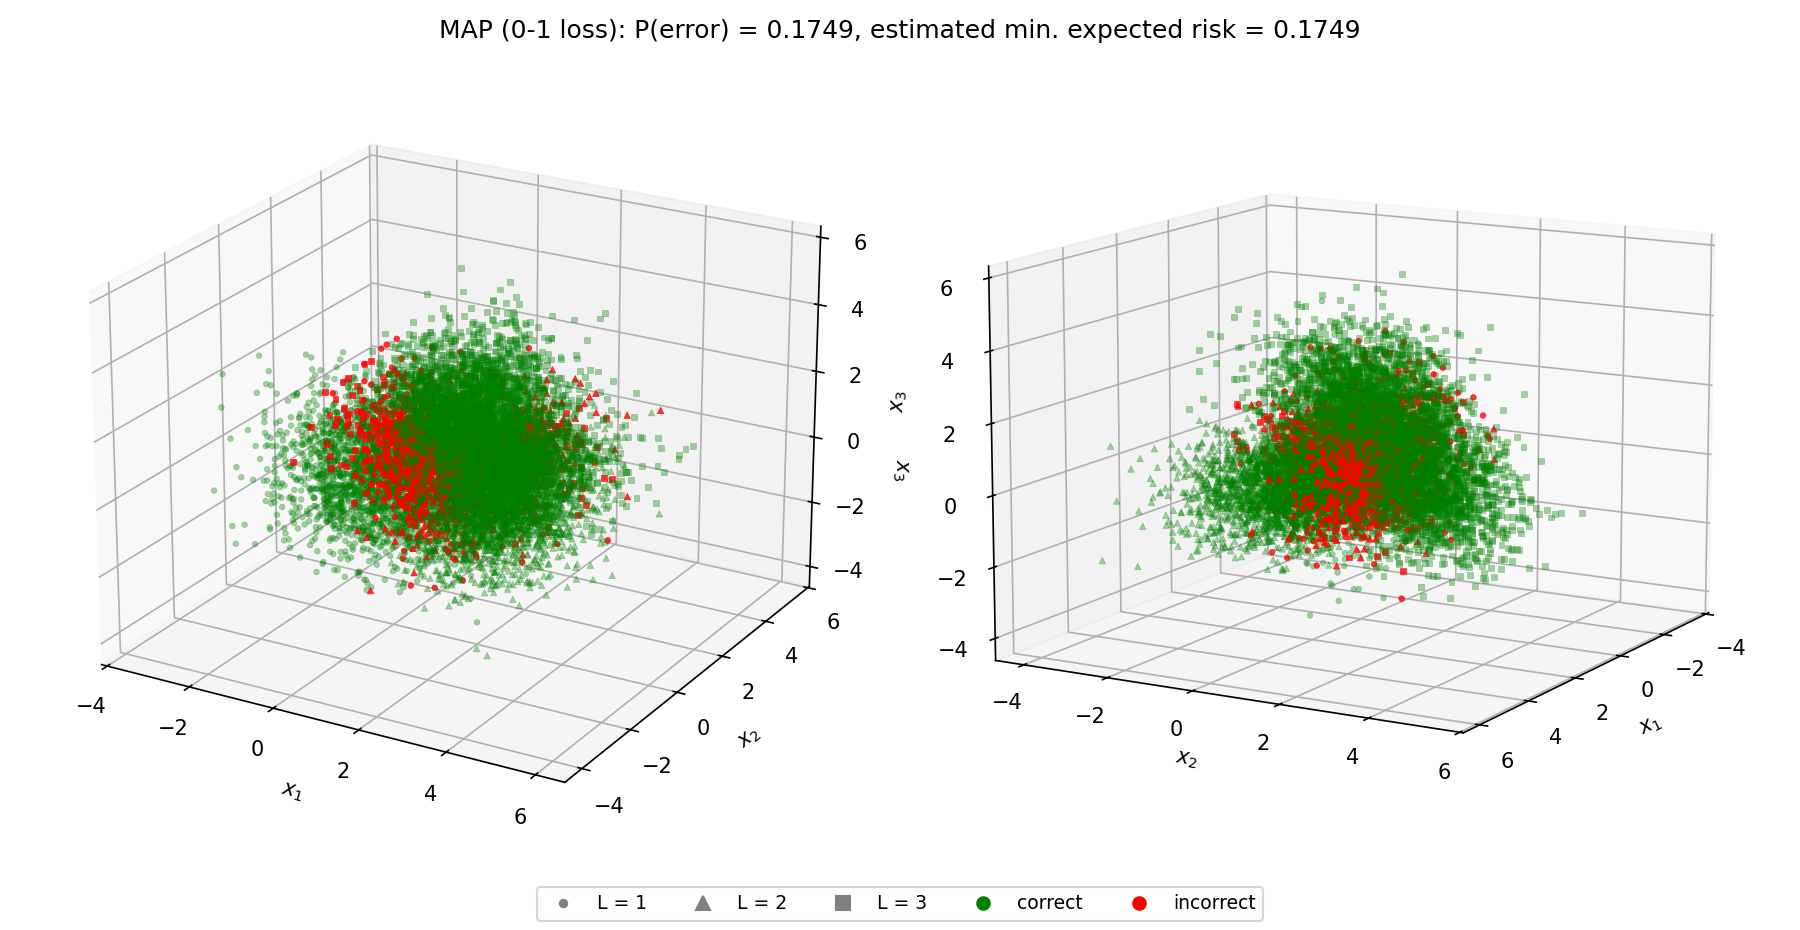
\includegraphics[width=0.92\linewidth]{figs/q2_scatter_01.png}
\caption{MAP classification of the 10K samples, two viewing angles.}\label{fig:q2a}
\end{figure}

\subsection*{Part B: ERM with $\Lambda_{10}$ and $\Lambda_{100}$}
The ERM rule is $D(\x)=\arg\min_i\sum_j\lambda_{ij}P(L{=}j|\x)$. For $\Lambda_w=\begin{bmatrix}0&1&w\\1&0&w\\1&1&0\end{bmatrix}$ (with $P_j\equiv P(L{=}j|\x)$):
\[
R(1|\x)=P_2+wP_3,\quad R(2|\x)=P_1+wP_3,\quad R(3|\x)=P_1+P_2=1-P_3 .
\]
Between 1 and 2 the $wP_3$ term cancels, so that choice is still by larger posterior. Class 3 is chosen iff $1-P_3<\min(P_1,P_2)+wP_3$, i.e.
\[
P(L{=}3|\x) > \frac{1-\min\{P(L{=}1|\x),P(L{=}2|\x)\}}{w+1}.
\]
The right side lies between $\tfrac{1}{2(w+1)}$ and $\tfrac1{w+1}$. So with $w=10$, class 3 is chosen once its posterior exceeds at most $1/11\approx0.09$; with $w=100$, once it exceeds at most $1/101\approx0.01$.

The minimum expected risk is estimated by the sample average of the loss actually incurred, $\hat R_{\min}=\frac1N\sum_n\lambda_{D(\x_n),L_n}$. A second, lower-variance estimate is $\frac1N\sum_n\min_iR(D{=}i|\x_n)$, which uses the true posteriors. Both agree closely:
\begin{center}\small\begin{tabular}{lccccc}
\toprule
Loss & $\hat{R}_{\min}=\frac1N\sum_n\lambda_{D_nL_n}$ & $\frac1N\sum_n \min_i R(D{=}i|x_n)$ & $\hat P(\text{error})$ & \#$\{D=1,2,3\}$ \\
\midrule
0--1 & 0.1749 & 0.1775 & 0.1749 & 2893, 2897, 4210 \\
$\Lambda_{10}$ & 0.3387 & 0.3451 & 0.2757 & 1567, 1933, 6500 \\
$\Lambda_{100}$ & 0.4882 & 0.4899 & 0.4387 & 550, 1063, 8387 \\
\bottomrule
\end{tabular}
\end{center}

\noindent Confusion matrices $\hat P(D{=}i|L{=}j)$ for $\Lambda_{10}$ and $\Lambda_{100}$, respectively:
\begin{center}\small
\begin{tabular}{lrrr}
\toprule
 & $L=1$ & $L=2$ & $L=3$ \\
\midrule
$D=1$ & \textbf{0.4912} (1449) & 0.0267 (80) & 0.0094 (38) \\
$D=2$ & 0.0319 (94) & \textbf{0.6037} (1807) & 0.0079 (32) \\
$D=3$ & 0.4769 (1407) & 0.3695 (1106) & \textbf{0.9827} (3987) \\
\bottomrule
\end{tabular}
\quad
\begin{tabular}{lrrr}
\toprule
 & $L=1$ & $L=2$ & $L=3$ \\
\midrule
$D=1$ & \textbf{0.1797} (530) & 0.0060 (18) & 0.0005 (2) \\
$D=2$ & 0.0098 (29) & \textbf{0.3445} (1031) & 0.0007 (3) \\
$D=3$ & 0.8105 (2391) & 0.6495 (1944) & \textbf{0.9988} (4052) \\
\bottomrule
\end{tabular}

\end{center}

\begin{figure}[H]\centering
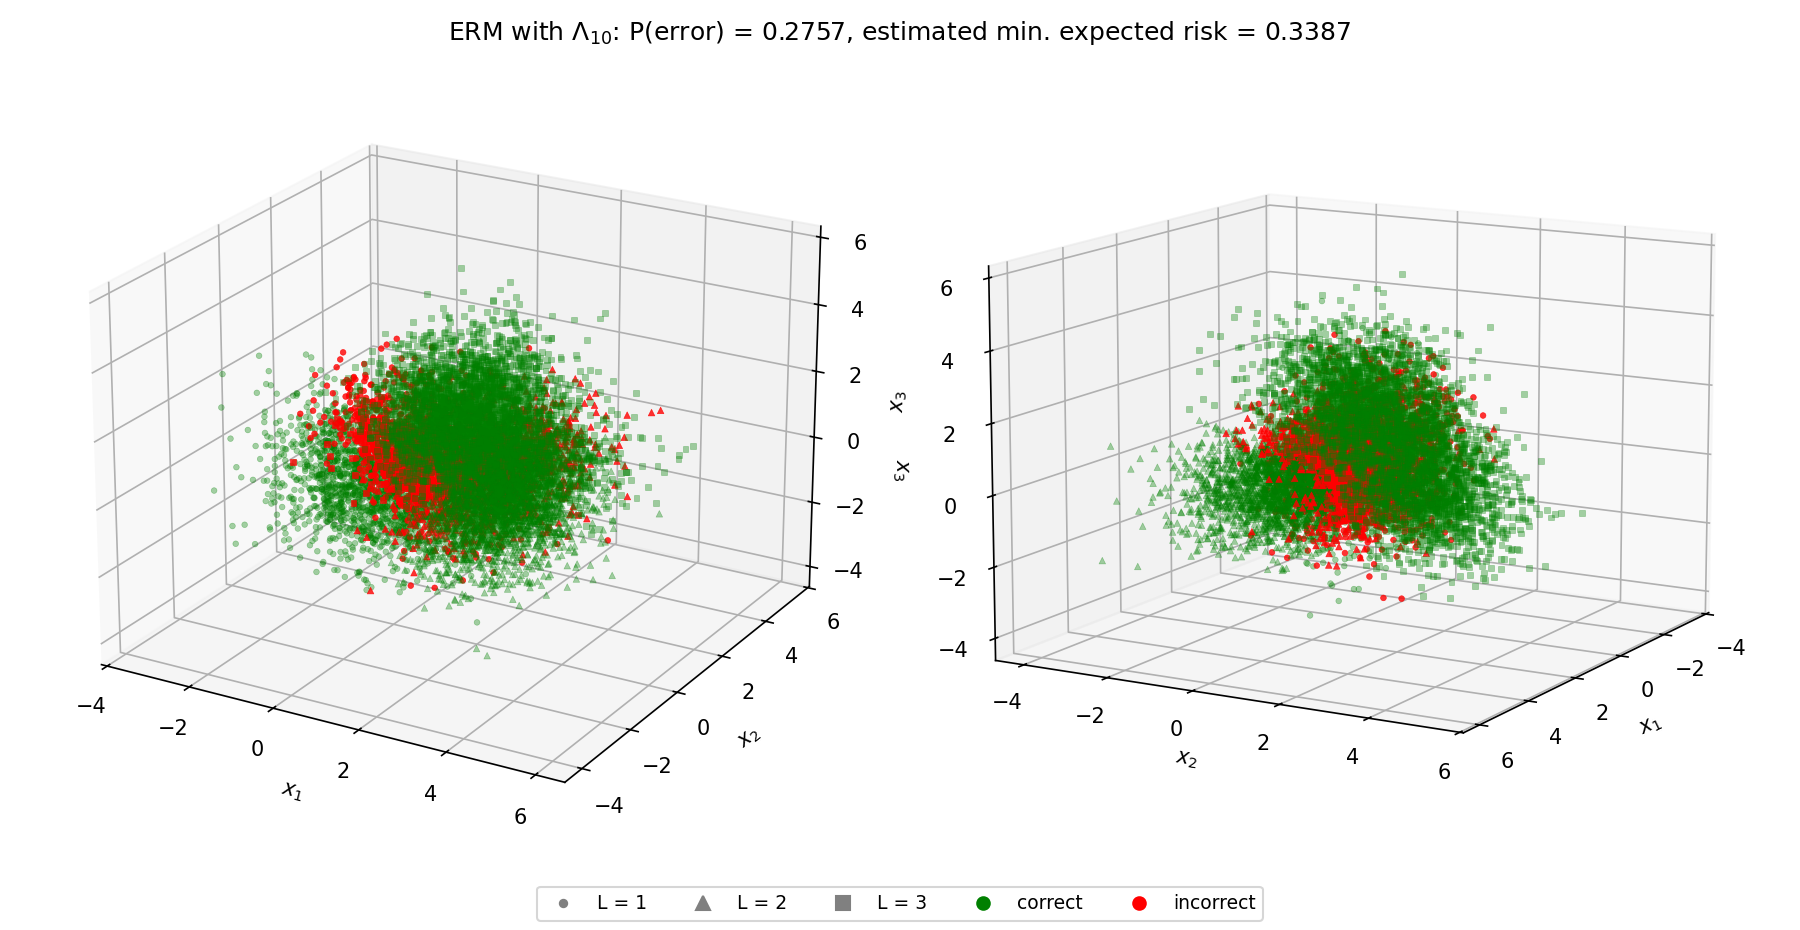
\includegraphics[width=0.49\linewidth]{figs/q2_scatter_10.png}\hfill
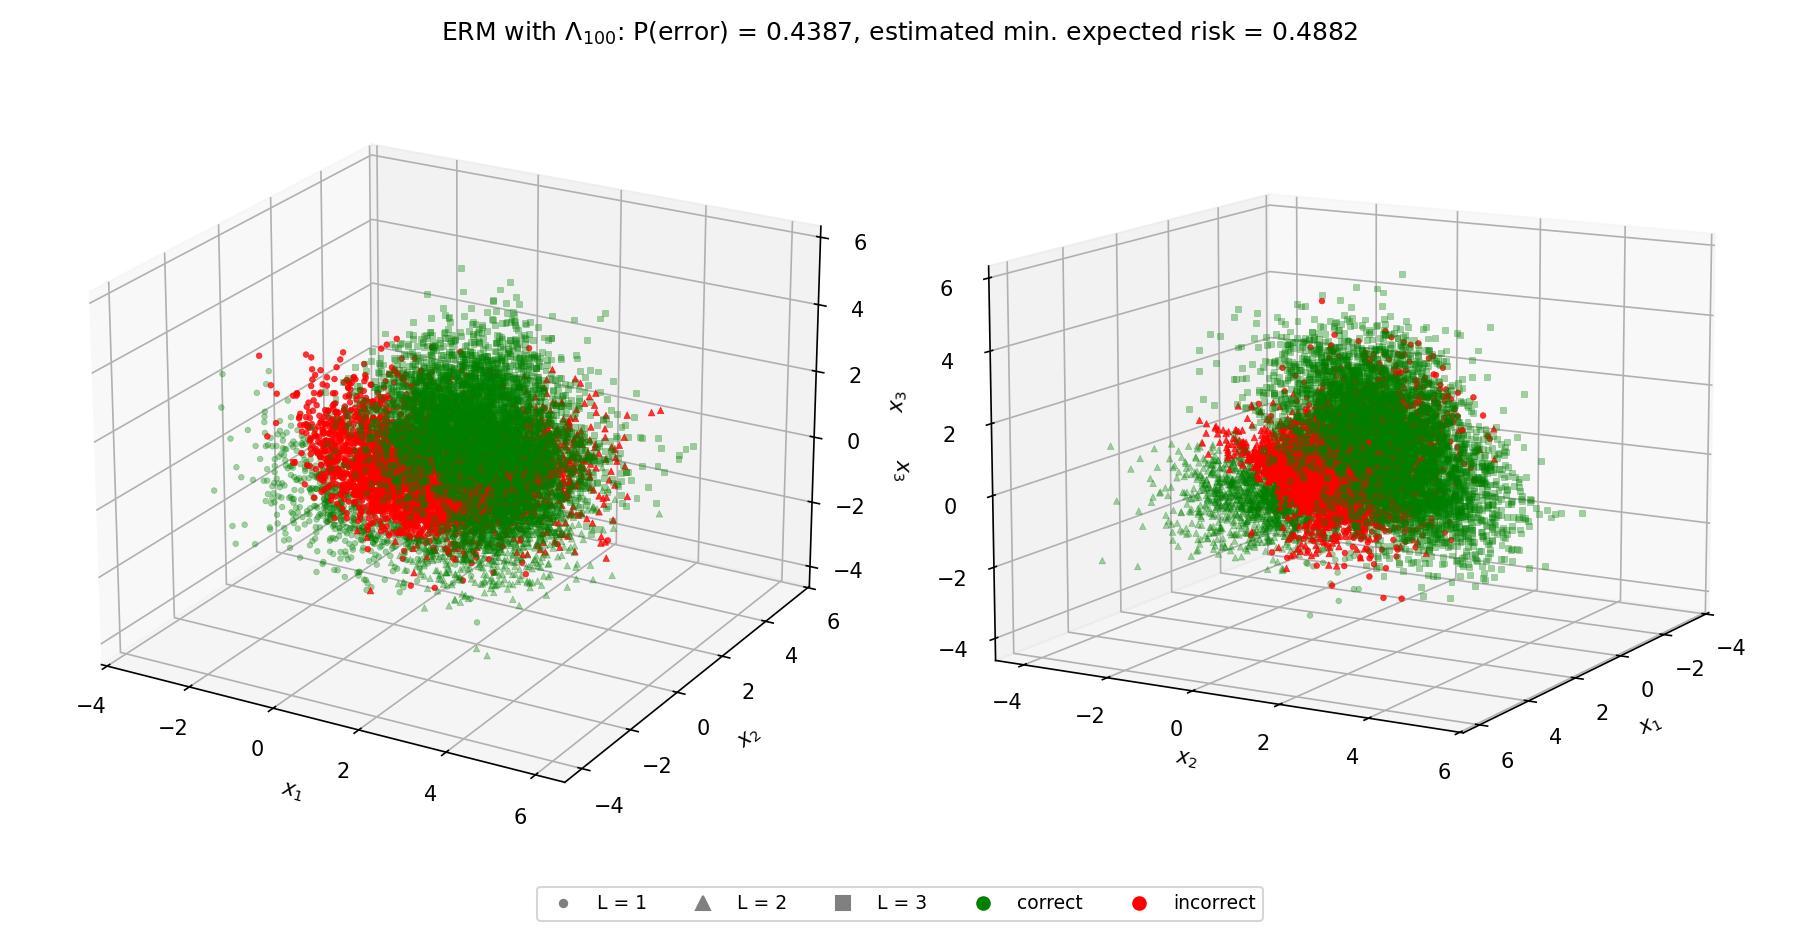
\includegraphics[width=0.49\linewidth]{figs/q2_scatter_100.png}
\caption{ERM decisions with $\Lambda_{10}$ (left) and $\Lambda_{100}$ (right); same marker/colour convention as Fig.~\ref{fig:q2a}.}\label{fig:q2b}
\end{figure}

\begin{figure}[H]\centering
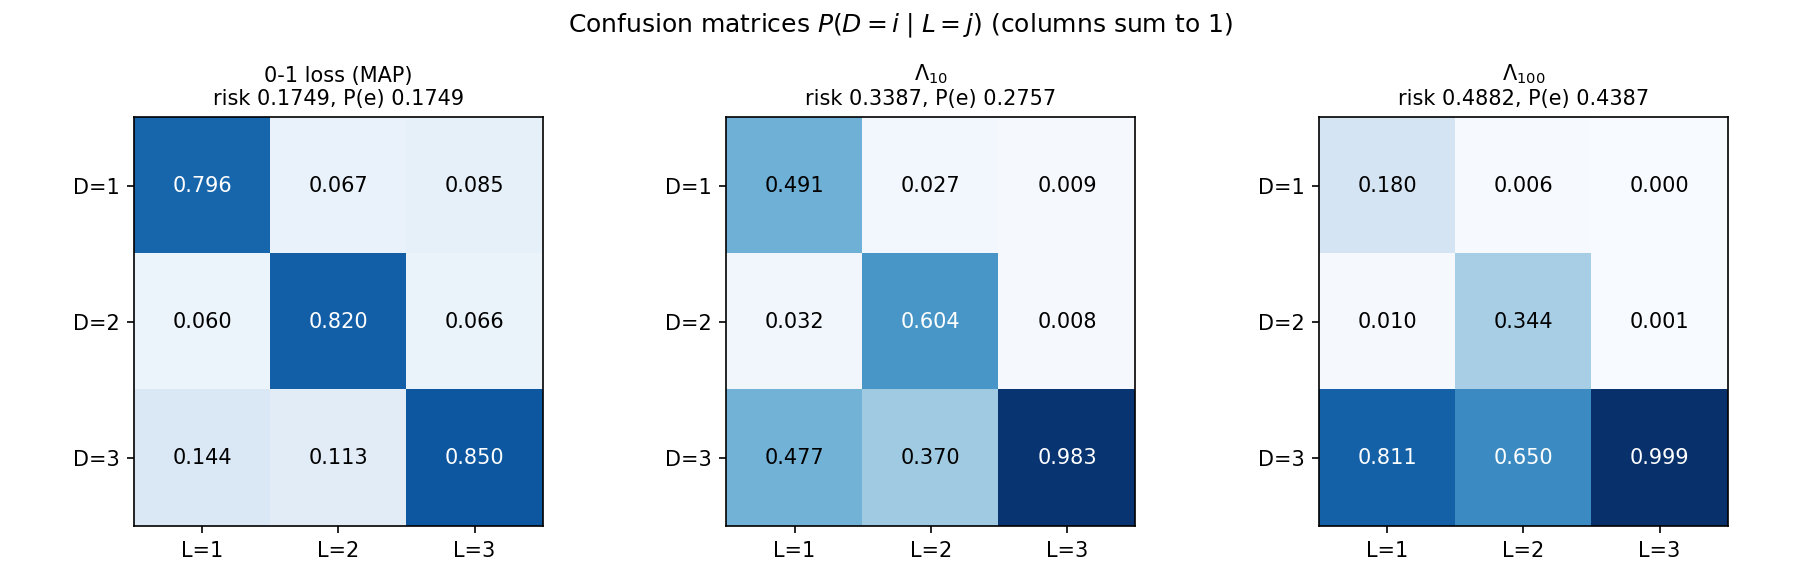
\includegraphics[width=0.85\linewidth]{figs/q2_confusions.png}\\
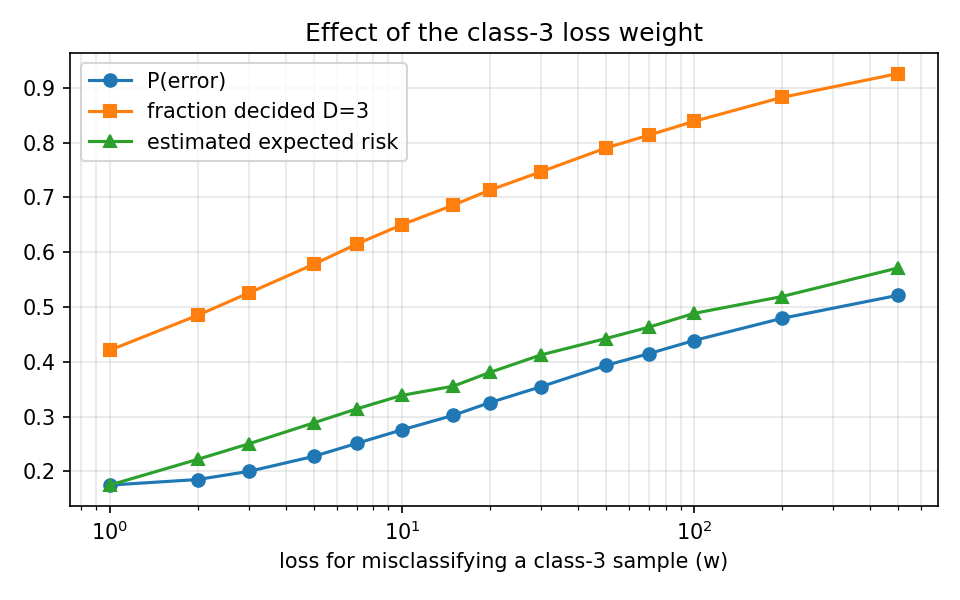
\includegraphics[width=0.55\linewidth]{figs/q2_sweep.png}
\caption{Top: confusion matrices for the three loss matrices. Bottom: P(error), fraction of $D=3$ decisions, and estimated expected risk as the class-3 loss weight $w$ varies from 1 (0--1 loss) to 500.}\label{fig:q2c}
\end{figure}

\textbf{Insights.}
\begin{itemize}
\item \emph{Risk vs.\ error.} As $w$ grows, ERM trades many cheap errors for few expensive ones. Class-3 recall goes $0.850\to0.983\to0.999$, while recall of classes 1 and 2 collapses ($0.796\to0.491\to0.180$ and $0.820\to0.604\to0.345$). The number of $D=3$ decisions rises from 4210 to 6500 to 8387. $P(\text{error})$ rises sharply ($0.175\to0.276\to0.439$), but this is the risk-optimal behaviour, not a failure.
\item \emph{Minimum risk grows with $w$} ($0.175\to0.339\to0.488$): larger penalties cannot reduce the best achievable risk. However, the growth is strongly sub-linear in $w$ because the classifier adapts. Under $\Lambda_{100}$ only 5 of 4057 class-3 samples are missed, yet those 5 still contribute $500/10^4=0.05$ to the risk. The 4335 class-1/2 observations assigned class 3 contribute $0.4335$, and 47 class-1/2 cross-errors contribute $0.0047$, giving total risk $0.4882$.
\item \emph{Asymmetry between classes 1 and 2:} class 1 loses more recall than class 2. Because of the covariance orientations, more of class 1's probability mass lies where $P(L{=}3|\x)$ exceeds the low class-3 threshold.
\item In the limit $w\to\infty$ the rule degenerates to ``always decide 3'', with risk $0.6$ (all class-1/2 samples wrong at cost 1). The sweep shows the risk approaching that value (0.571 at $w=500$).
\end{itemize}

%==========================================================================
\clearpage\section*{Question 3: Estimated Gaussian class models}

\subsection*{Model, estimators and decision rule}
For each dataset with classes $j\in\mathcal{C}$ and samples $\{(\x_n,L_n)\}_{n=1}^N$, $\x_n\in\mathbb{R}^d$:
\begin{enumerate}
\item \textbf{Assumptions.} Samples are i.i.d.; the class-conditional pdf of each class is a single multivariate Gaussian, $p(\x|L{=}j)=g(\x|\m_j,C_j)$, with its own full covariance (heteroscedastic, i.e.\ a quadratic-discriminant model). No independence between features is assumed.
\item \textbf{Preprocessing.} For the required all-sample fit, each feature is z-scored with the mean and standard deviation of all samples, $\tilde x_k=(x_k-\bar x_k)/s_k$. An invertible affine map changes every $\ln p(\x|j)$ by the same constant (the log-Jacobian) and leaves an \emph{unregularized} Gaussian classifier's decisions unchanged. Regularization with $\lambda I$ is \emph{not} affine-invariant, though, and wine features differ in variance by $\sim10^8$ (e.g.\ total SO$_2$ vs.\ density). Standardizing makes $\lambda I$ an isotropic shrinkage in comparable units. Without it, the same classifier on raw wine features has training error $0.600$ instead of $0.503$, because $\lambda$ swamps the small-variance features. When tuning $\alpha$ (below), the mean and standard deviation are estimated on the training portion only and then applied to the validation portion, so no validation data leak into the fitted model.
\item \textbf{Estimates (maximum likelihood / sample averages).} $\hat P(L{=}j)=N_j/N$; $\hat\m_j=\frac1{N_j}\sum_{n:L_n=j}\x_n$; $\hat C_j=\frac1{N_j}\sum_{n:L_n=j}(\x_n-\hat\m_j)(\x_n-\hat\m_j)^T$.
\item \textbf{Regularization} (per class, following the hint): $C_j^{reg}=\hat C_j+\lambda_jI$ with $\lambda_j=\alpha\,\tr(\hat C_j)/\operatorname{rank}(\hat C_j)$, the arithmetic mean of the nonzero eigenvalues scaled by $\alpha$. All eigenvalues of $C_j^{reg}$ are then at least $\lambda_j>0$.
\item \textbf{Decision rule} (0--1 loss, MAP): $D(\x)=\arg\max_j\big[-\tfrac12(\x-\hat\m_j)^T(C_j^{reg})^{-1}(\x-\hat\m_j)-\tfrac12\ln|C_j^{reg}|+\ln\hat P(L{=}j)\big]$, evaluated with Cholesky factors.
\item \textbf{Choosing $\alpha$.} Training error reuses the fitting observations and can favor overfitting; it is not a reliable criterion for generalization. It need not decrease monotonically as $\alpha$ decreases. I therefore selected $\alpha$ on validation data and then, as the assignment requires, re-estimated all parameters on all samples and report the all-sample (training) error and confusion matrix. Wine: stratified 5-fold cross-validation, giving $\alpha=10^{-3}$ (CV error is flat, about 0.515, for all $\alpha\le10^{-2}$). HAR: the dataset's own subject-disjoint train/test split, used here as a validation split (train on the 7352 training samples, score the 2947 others), giving $\alpha=10^{-4}$. Because this split chose $\alpha$, its score is a validation score, not an untouched test score; no separate final test was performed. The sweep is in Table~\ref{tab:sweep} and Fig.~\ref{fig:sweep}.
\end{enumerate}

\begin{table}[H]\centering\small
\begin{tabular}{lcccc}
\toprule
$\alpha$ & Wine: training & Wine: 5-fold CV & HAR: training & HAR: validation \\
\midrule
1e-06 & 0.5002 & 0.5155 & 0.0217 & 0.0845 \\
1e-05 & 0.5002 & 0.5155 & 0.0118 & 0.0821 \\
0.0001 & 0.5008 & 0.5157 & 0.0030 & 0.0818 \\
0.001 & 0.5033 & 0.5149 & 0.0149 & 0.1035 \\
0.01 & 0.5043 & 0.5184 & 0.0652 & 0.1256 \\
0.03 & 0.5065 & 0.5214 & 0.0938 & 0.1354 \\
0.1 & 0.5159 & 0.5296 & 0.1482 & 0.1927 \\
0.3 & 0.5208 & 0.5300 & 0.2633 & 0.3156 \\
\bottomrule
\end{tabular}

\caption{P(error) versus regularization strength $\alpha$.}\label{tab:sweep}
\end{table}
\begin{figure}[H]\centering
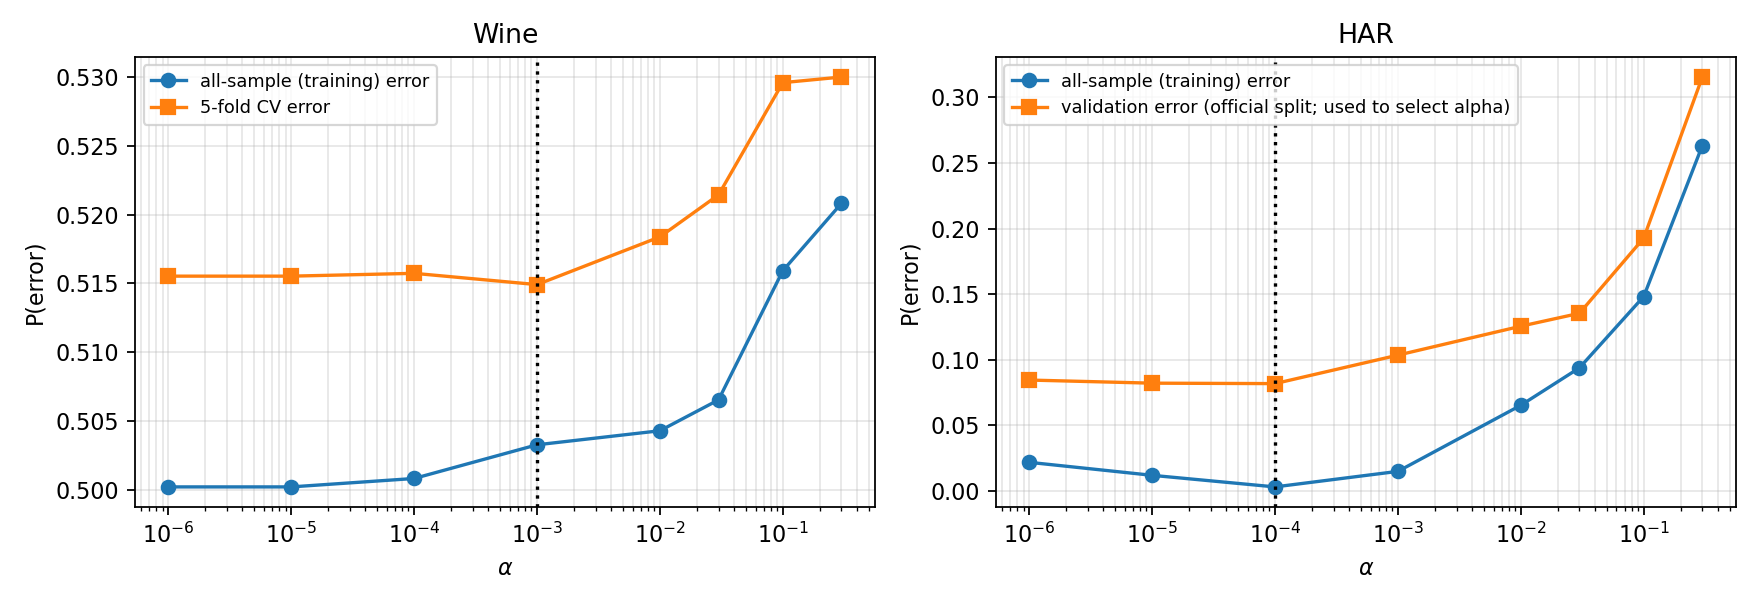
\includegraphics[width=0.85\linewidth]{figs/q3_alpha_sweep.png}
\caption{Effect of $\alpha$; dotted line = selected value.}\label{fig:sweep}
\end{figure}

\subsection*{Results: Wine Quality (white, $N=4898$, $d=11$)}
Seven quality levels occur (3--9); levels 0--2 and 10 have no samples and are therefore not classes of the model. Per-class estimates:
\begin{center}\small\begin{tabular}{lrrrrrr}
\toprule
Class & $N_j$ & $\hat P(L{=}j)$ & rank$(\hat C_j)$ & $\lambda_j$ & cond$(\hat C_j)$ & cond$(\hat C_j+\lambda_j I)$ \\
\midrule
3 & 20 & 0.0041 & 11 & 3.47e-03 & 1.31e+03 & 1.07e+03 \\
4 & 163 & 0.0333 & 11 & 1.36e-03 & 1.54e+02 & 1.47e+02 \\
5 & 1457 & 0.2975 & 11 & 9.93e-04 & 2.18e+02 & 2.03e+02 \\
6 & 2198 & 0.4488 & 11 & 9.37e-04 & 1.11e+02 & 1.07e+02 \\
7 & 880 & 0.1797 & 11 & 7.71e-04 & 3.06e+02 & 2.83e+02 \\
8 & 175 & 0.0357 & 11 & 8.86e-04 & 5.42e+02 & 4.74e+02 \\
9 & 5 & 0.0010 & 4 & 1.28e-03 & 6.63e+17 & 2.54e+03 \\
\bottomrule
\end{tabular}
\end{center}
Class 9 has only 5 samples in 11 dimensions, so $\hat C_9$ has rank 4 and is singular (condition number $\sim10^{17}$). Regularization is mandatory here; the other classes are well conditioned.

\textbf{Estimated $P(\text{error})=\mathbf{0.5033}$} ($\alpha=10^{-3}$, all samples). Confusion matrix $\hat P(D{=}i|L{=}j)$:
\begin{center}\small\begin{tabular}{lrrrrrrr}
\toprule
 & $L=3$ & $L=4$ & $L=5$ & $L=6$ & $L=7$ & $L=8$ & $L=9$ \\
\midrule
$D=3$ & \textbf{0.450} & 0.018 & 0.006 & 0.002 & 0.000 & 0.000 & 0.000 \\
$D=4$ & 0.050 & \textbf{0.233} & 0.036 & 0.012 & 0.002 & 0.000 & 0.000 \\
$D=5$ & 0.150 & 0.417 & \textbf{0.570} & 0.221 & 0.032 & 0.017 & 0.000 \\
$D=6$ & 0.200 & 0.252 & 0.279 & \textbf{0.405} & 0.216 & 0.280 & 0.000 \\
$D=7$ & 0.100 & 0.074 & 0.107 & 0.353 & \textbf{0.733} & 0.617 & 0.000 \\
$D=8$ & 0.050 & 0.006 & 0.001 & 0.007 & 0.017 & \textbf{0.086} & 0.000 \\
$D=9$ & 0.000 & 0.000 & 0.000 & 0.000 & 0.000 & 0.000 & \textbf{1.000} \\
\bottomrule
\end{tabular}
\end{center}
For reference: always guessing the majority class (6) gives error $0.551$; predicting within $\pm1$ grade succeeds for $92.7\%$ of samples.

\begin{figure}[H]\centering
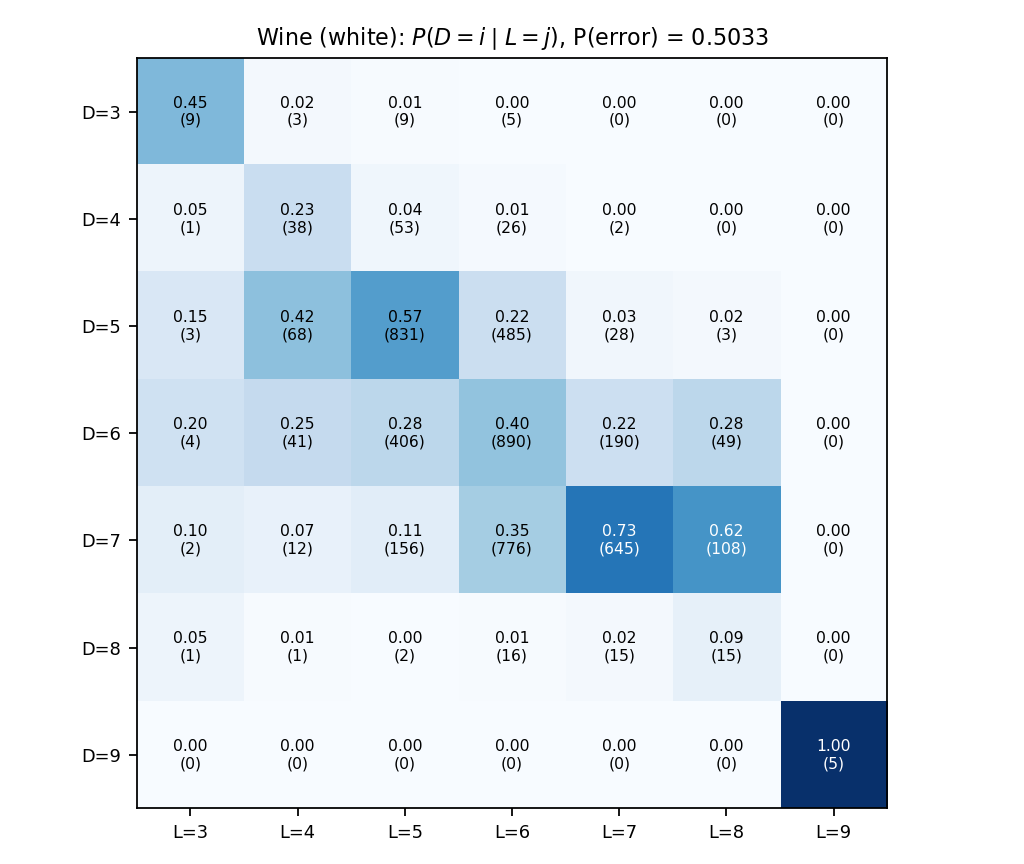
\includegraphics[width=0.5\linewidth]{figs/q3_wine_conf.png}
\caption{Wine confusion matrix (counts in parentheses).}
\end{figure}

\subsection*{Results: Human Activity Recognition ($N=10299$, $d=561$)}
\begin{center}\small\begin{tabular}{lrrrrrr}
\toprule
Class & $N_j$ & $\hat P(L{=}j)$ & rank$(\hat C_j)$ & $\lambda_j$ & cond$(\hat C_j)$ & cond$(\hat C_j+\lambda_j I)$ \\
\midrule
1 Walk & 1722 & 0.1672 & 468 & 7.35e-05 & 7.0e+34 & 1.15e+06 \\
2 Up & 1544 & 0.1499 & 468 & 6.48e-05 & 3.1e+35 & 9.19e+05 \\
3 Down & 1406 & 0.1365 & 469 & 1.21e-04 & 1.6e+34 & 1.50e+06 \\
4 Sit & 1777 & 0.1725 & 468 & 3.80e-05 & 1.9e+34 & 1.15e+06 \\
5 Stand & 1906 & 0.1851 & 468 & 3.22e-05 & 7.6e+33 & 9.57e+05 \\
6 Lay & 1944 & 0.1888 & 468 & 4.96e-05 & 6.8e+34 & 1.05e+06 \\
\bottomrule
\end{tabular}
\end{center}
Every class covariance has numerical rank 468--469 although each class has more observations than features. The numerical rank shows strong linear redundancy among the 561 engineered features (many are derived from the same underlying signals); the specific relationships were not analysed. The raw $\hat C_j$ are therefore numerically singular (condition numbers $\sim10^{35}$). Regularization brings them to $\sim10^6$.

\textbf{Estimated $P(\text{error})=\mathbf{0.0030}$} ($\alpha=10^{-4}$, all samples, 31 errors). Confusion matrix:
\begin{center}\small\begin{tabular}{lrrrrrr}
\toprule
 & $L$=Walk & $L$=Up & $L$=Down & $L$=Sit & $L$=Stand & $L$=Lay \\
\midrule
$D$=Walk & \textbf{0.9994} & 0.0000 & 0.0000 & 0.0000 & 0.0000 & 0.0000 \\
$D$=Up & 0.0006 & \textbf{1.0000} & 0.0085 & 0.0000 & 0.0000 & 0.0000 \\
$D$=Down & 0.0000 & 0.0000 & \textbf{0.9915} & 0.0000 & 0.0000 & 0.0000 \\
$D$=Sit & 0.0000 & 0.0000 & 0.0000 & \textbf{0.9983} & 0.0079 & 0.0000 \\
$D$=Stand & 0.0000 & 0.0000 & 0.0000 & 0.0017 & \textbf{0.9921} & 0.0000 \\
$D$=Lay & 0.0000 & 0.0000 & 0.0000 & 0.0000 & 0.0000 & \textbf{1.0000} \\
\bottomrule
\end{tabular}
\end{center}
On the official split's second part (train on 7352 samples, score the other 2947, from different subjects) the same model has validation error $0.082$. This is optimistic as a test estimate, because the same split chose $\alpha$.

\begin{figure}[H]\centering
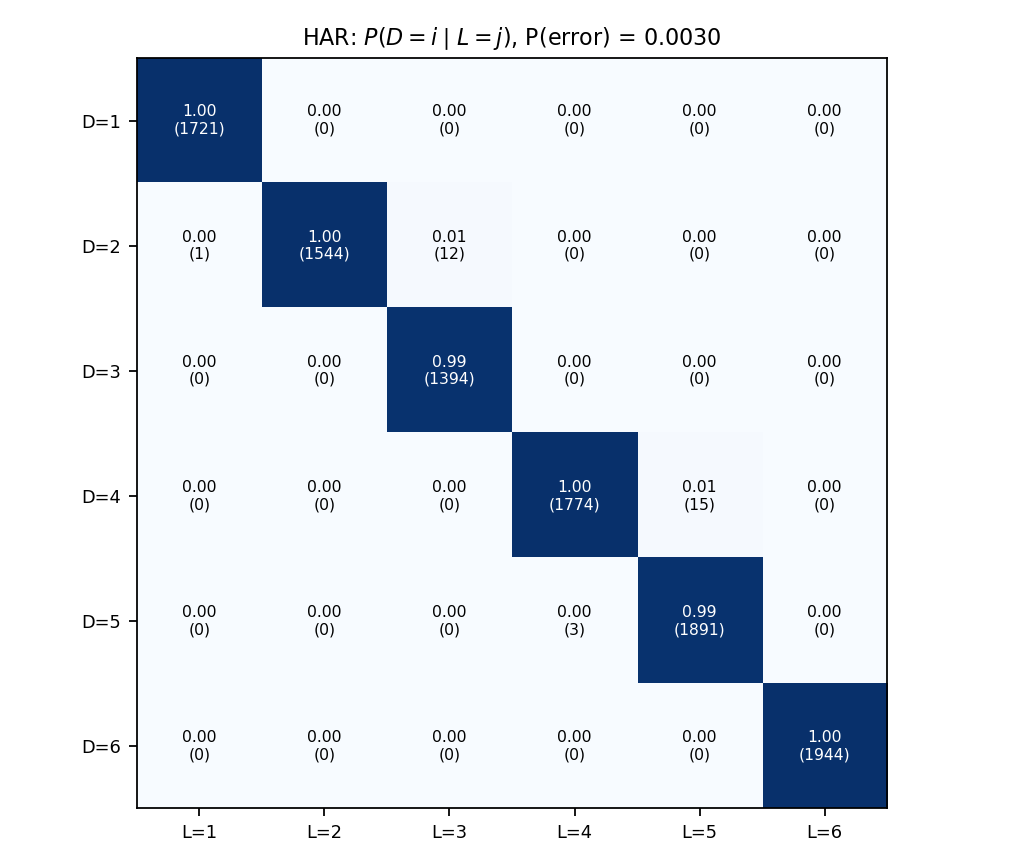
\includegraphics[width=0.5\linewidth]{figs/q3_har_conf.png}
\caption{HAR confusion matrix (counts in parentheses).}
\end{figure}

\subsection*{Visualizations}
\begin{figure}[H]\centering
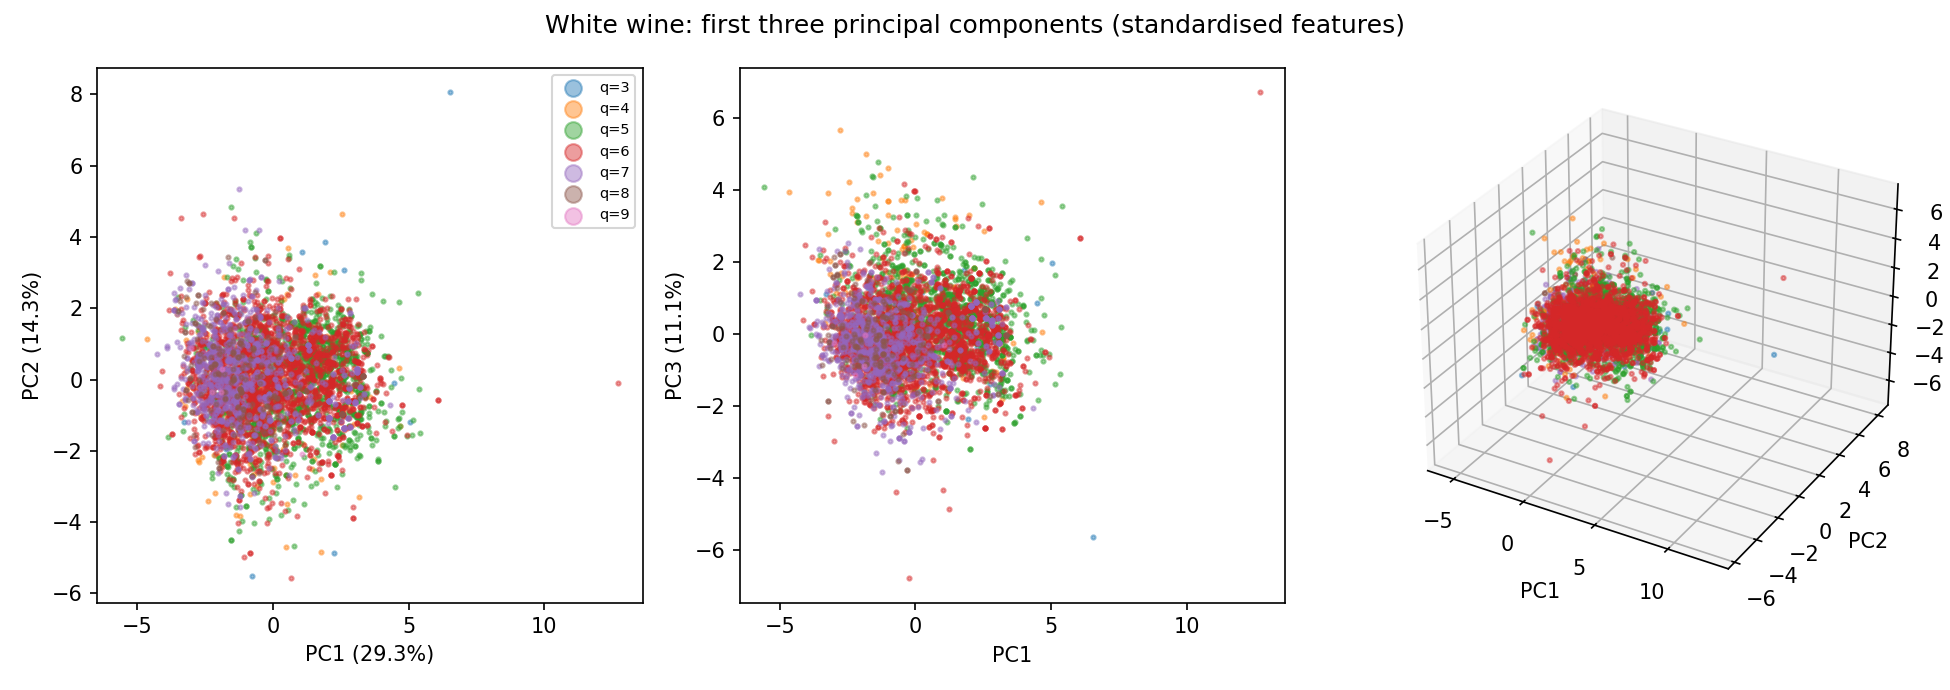
\includegraphics[width=\linewidth]{figs/q3_wine_pca.png}
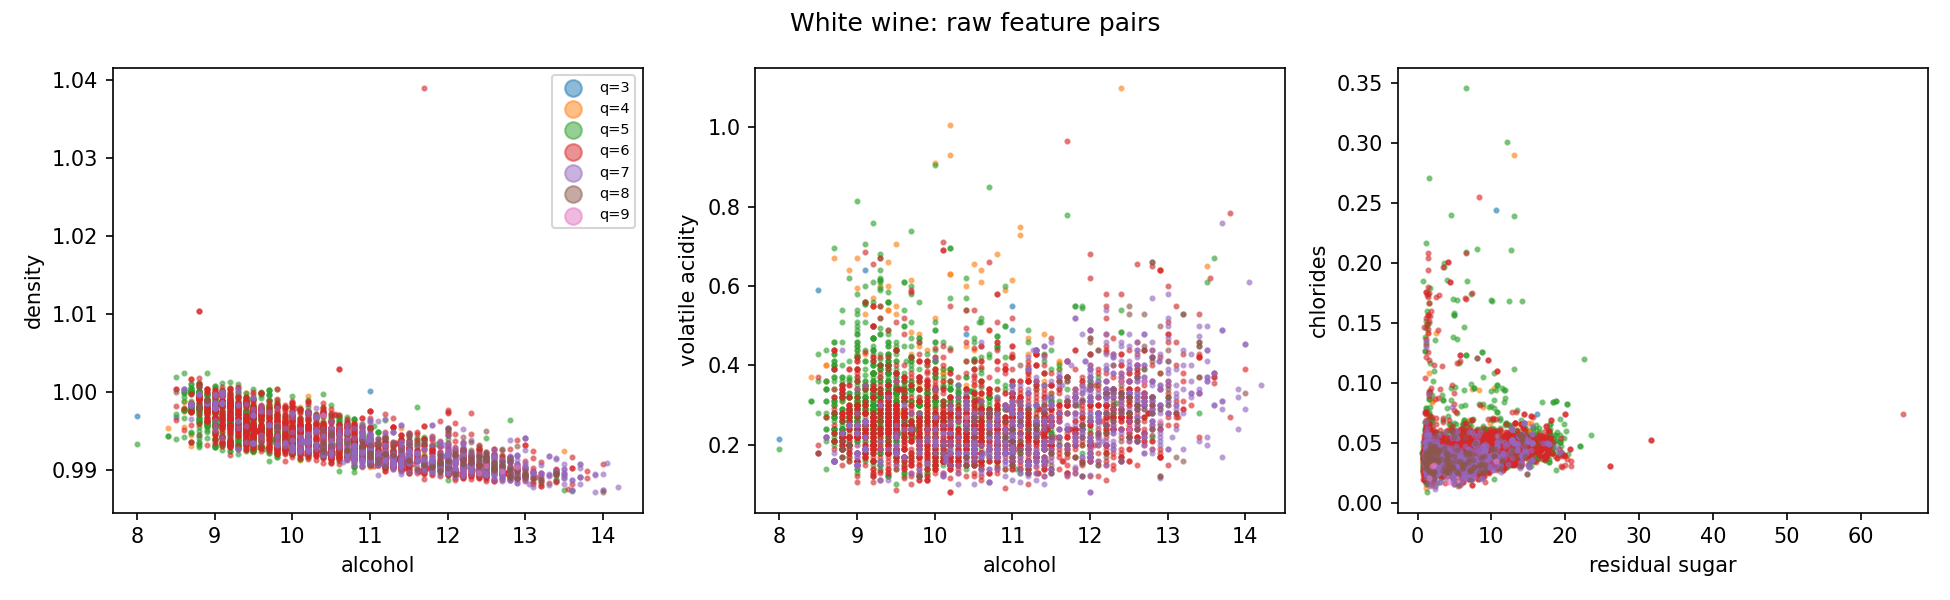
\includegraphics[width=\linewidth]{figs/q3_wine_pairs.png}
\caption{Wine: first three principal components of the standardized features (PC1--3 explain 29\%, 14\%, 11\% of variance), and three raw feature pairs.}\label{fig:winevis}
\end{figure}
\begin{figure}[H]\centering
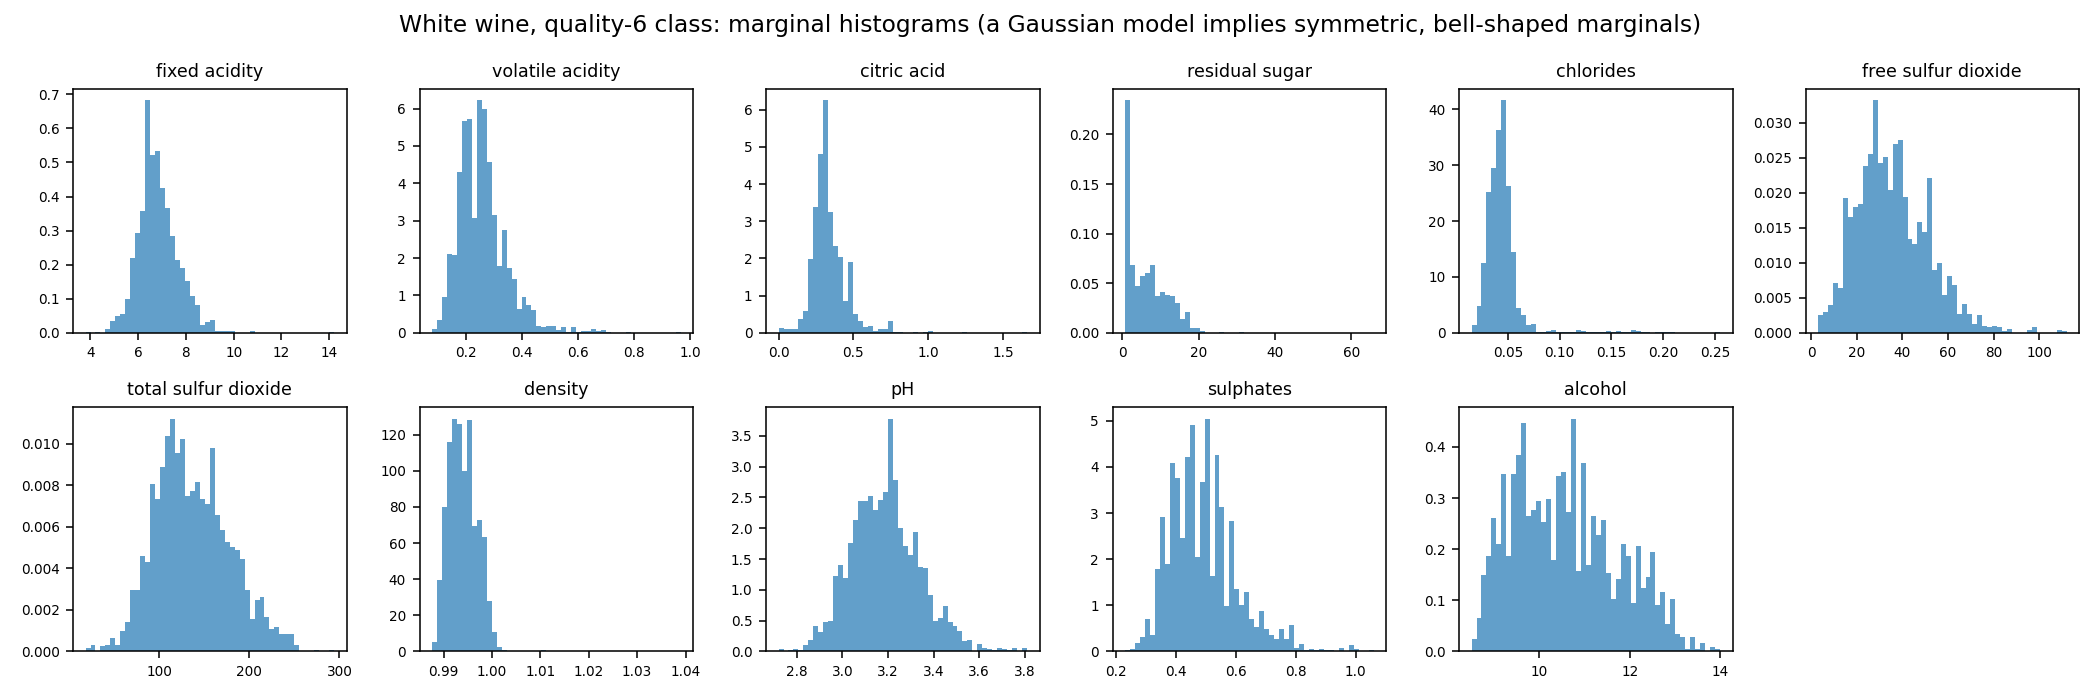
\includegraphics[width=\linewidth]{figs/q3_wine_hist.png}
\caption{Wine: marginal histograms of all 11 features within the quality-6 class.}\label{fig:winehist}
\end{figure}
\begin{figure}[H]\centering
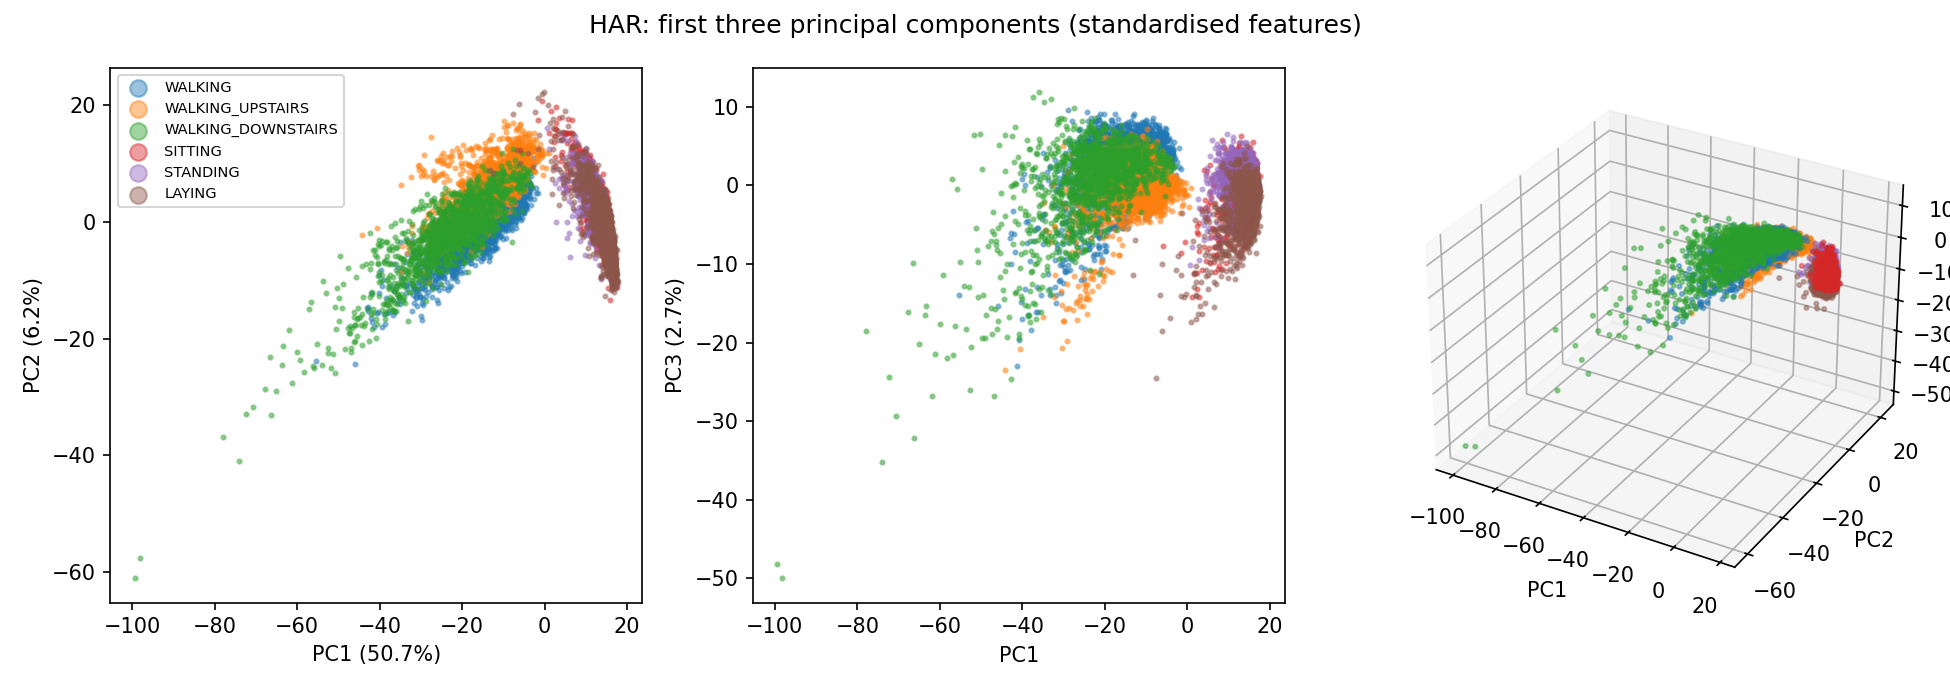
\includegraphics[width=\linewidth]{figs/q3_har_pca.png}
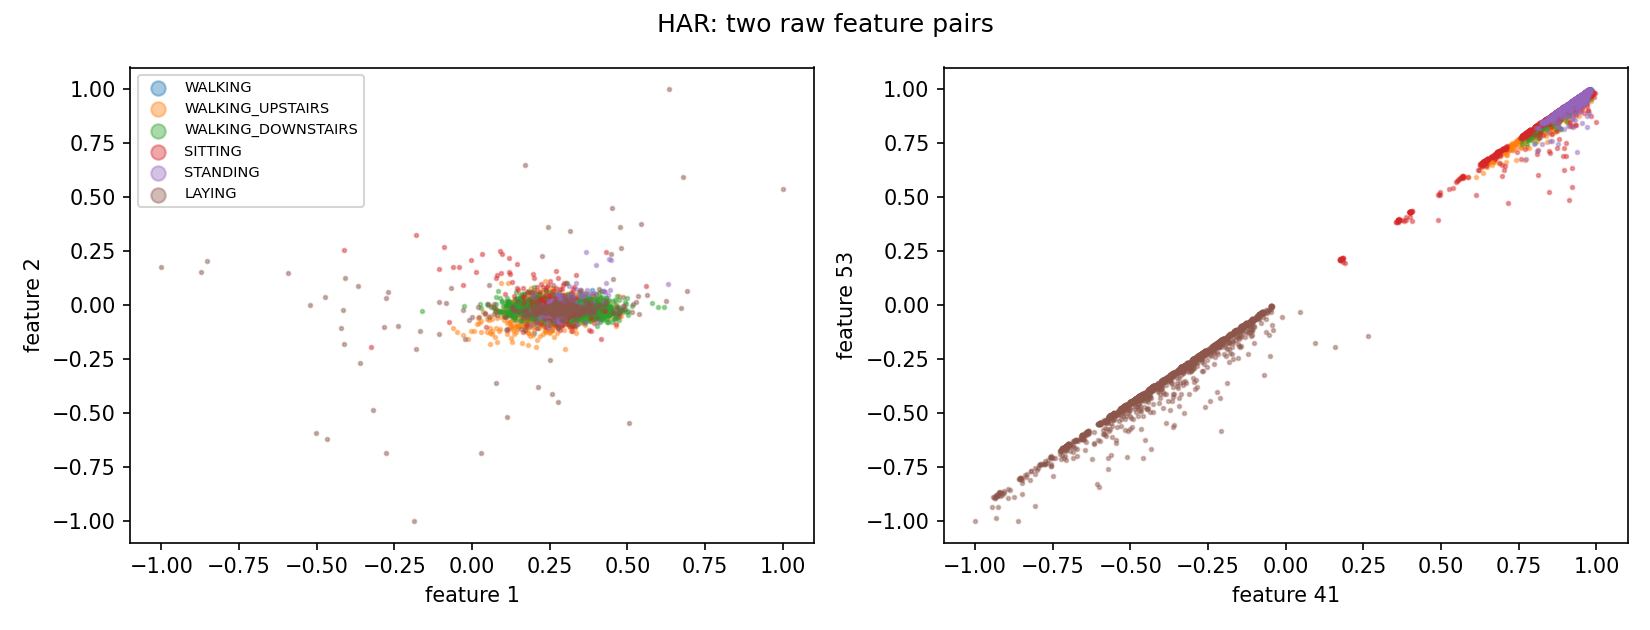
\includegraphics[width=0.85\linewidth]{figs/q3_har_pairs.png}
\caption{HAR: first three principal components (PC1 alone explains 50.7\% of variance) and two raw feature pairs.}\label{fig:harvis}
\end{figure}
\begin{figure}[H]\centering
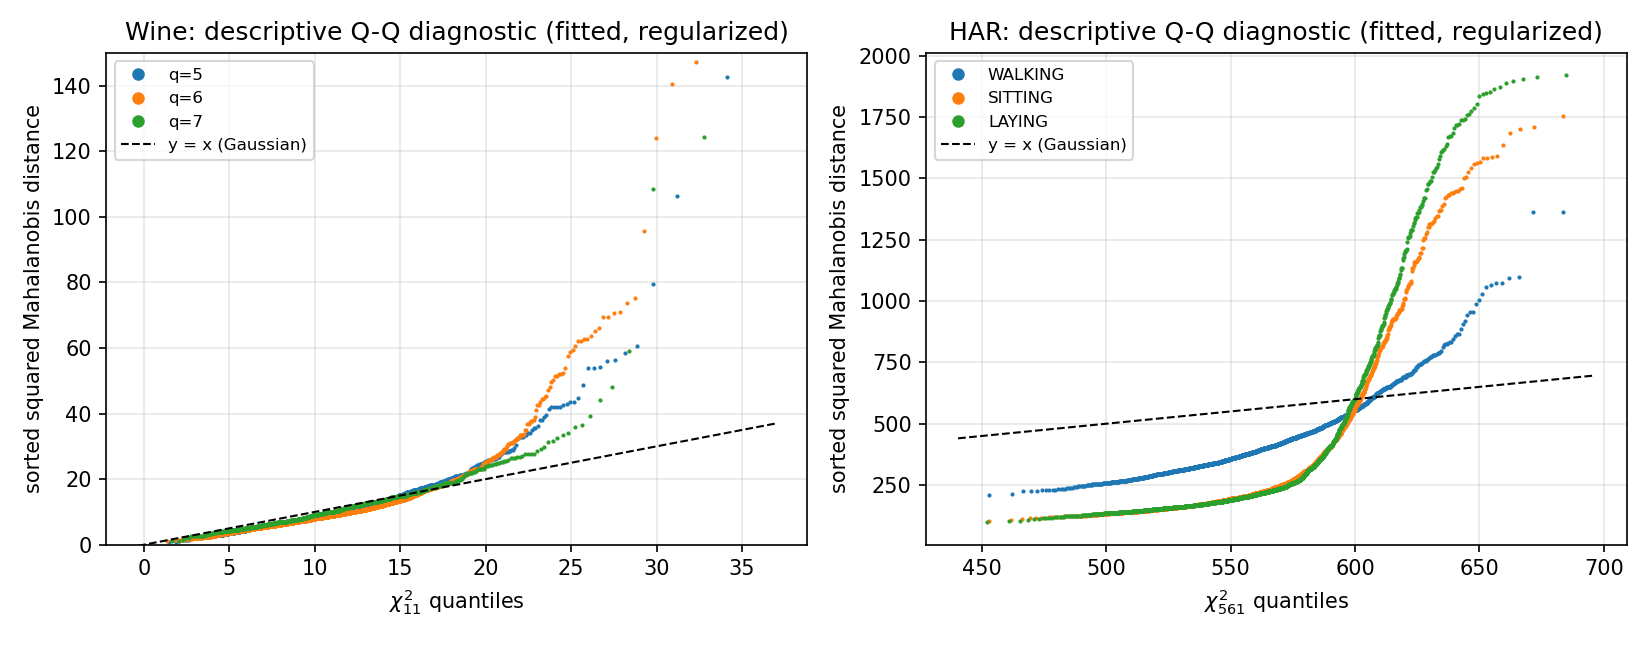
\includegraphics[width=\linewidth]{figs/q3_qq.png}
\caption{Gaussianity check (descriptive). If $\x\sim\mathcal N(\m_j,C_j)$, the squared Mahalanobis distance $r^2=(\x-\m_j)^TC_j^{-1}(\x-\m_j)\sim\chi^2_d$. The plot shows sorted $r^2$ (with the fitted, regularized model) against $\chi^2_d$ quantiles; with known, full-rank Gaussian parameters the population reference is the dashed line. Fitting, regularization, and numerical rank deficiency alter that reference; this figure is descriptive, not a calibrated goodness-of-fit test.}\label{fig:qq}
\end{figure}

\subsection*{Discussion: are Gaussian class conditionals appropriate?}

\textbf{Wine --- poorly, and the problem itself is hard.}
\begin{itemize}
\item \emph{Non-Gaussian features.} Several marginals are strongly right-skewed or heavy-tailed (residual sugar, chlorides, free SO$_2$, volatile acidity; Fig.~\ref{fig:winehist}). The Q-Q plot (Fig.~\ref{fig:qq}, left) follows $\chi^2_{11}$ up to roughly the 80th percentile, then shows much heavier tails: large distances suggest heavy tails, but fitted and regularized distances do not follow the nominal reference exactly. Transformations or mixture/robust models are plausible alternatives that would require separate evaluation.
\item \emph{Overlap.} In every projection (Fig.~\ref{fig:winevis}) the quality classes overlap almost completely and differ mostly by small mean shifts along alcohol/density. The labels are subjective, ordinal taster scores, which may limit predictability. These experiments do not estimate the true Bayes error; the fitted confusion matrix shows that nearly all errors are to adjacent grades (within $\pm1$: 92.7\%), and the Gaussian model's $P(\text{error})\approx0.50$ is only modestly better than the majority-class baseline (0.55).
\item \emph{How the model shaped the confusion matrix.} With near-identical means, the quadratic rule is driven largely by covariance differences and priors. Class 6 is the largest class (prior 0.45) but has only 40.5\% recall; 22\% and 35\% of its samples are assigned to the neighbouring grades 5 and 7, whose Gaussians overlap it almost completely. Rare grades are handled very differently. Class 9 (5 samples) gets a tiny, regularized Gaussian that recognizes its own 5 training points (5/5 correct), which is consistent with overfitting and provides little evidence about unseen quality-9 observations. Class 3 (20 samples) gets 45\% recall on training data. With 77 parameters per class ($11+66$), these rare-class estimates have very high variance, and their training-set performance is not trustworthy. CV error (0.515) slightly above the training error (0.503) shows a modest measured gap, without establishing the extent of overfitting for every class.
\end{itemize}

\textbf{HAR --- not Gaussian, but the classes are so well separated that a Gaussian quadratic classifier still works very well.}
\begin{itemize}
\item \emph{Non-Gaussianity.} The features are bounded in $[-1,1]$ by construction and come from many subjects, so each class may combine subject-specific distributions. The Q-Q plot (Fig.~\ref{fig:qq}, right) is far from $\chi^2_{561}$: distances are too small for most samples (the data effectively live in a $\approx468$-dimensional subspace, while regularization changes the distance metric) and far too large in the tail. The plot is descriptive, not a calibrated test: fitting, shrinkage and numerical rank deficiency can themselves produce departures from the nominal reference. The bounded features and heterogeneous activity structure also make an exact Gaussian model implausible; the plot alone cannot separate these effects.
\item \emph{Separation.} PCA (Fig.~\ref{fig:harvis}) shows two groups split cleanly along PC1: dynamic activities (walking, upstairs, downstairs) and static ones (sitting, standing, laying). Laying is also distinct. The only confusions are within the static group (sitting$\leftrightarrow$standing: 18 samples) and within the dynamic group (12 downstairs and 1 walking sample decided as upstairs), exactly the physically similar pairs. In 561 dimensions, a quadratic boundary with class-specific covariances is flexible enough to separate these classes even though each class is not Gaussian.
\item \emph{Overfitting and the role of $\lambda$.} Each class model has $561+561\cdot562/2\approx158{,}000$ parameters estimated from $\sim1{,}700$ samples. The all-sample error of 0.30\% is therefore heavily optimistic: on the other subjects of the official split the validation error is 8.2\%. Table~\ref{tab:sweep} shows the bias--variance trade-off. Large $\alpha$ (strong shrinkage toward a spherical covariance) underfits (error grows to 26--32\% at $\alpha=0.3$). Tiny $\alpha$ leaves the smallest eigen-directions, which are poorly estimated, almost unregularized. Training error need not be monotone in $\alpha$ (here it is lowest at $\alpha=10^{-4}$), and validation error is best at intermediate $\alpha=10^{-4}$ to $10^{-5}$.
\end{itemize}

\textbf{Summary.} The minimum-$P(\text{error})$ rule is guaranteed optimal under the specified class densities and priors; model mismatch can remove that guarantee. For wine, model mismatch (skewed, heavy-tailed, almost fully overlapping classes) plus severe class imbalance yields $\approx50\%$ error concentrated between adjacent grades. For HAR, the Gaussian model is also mismatched, but the class-conditional densities are concentrated in different regions, so the induced quadratic boundaries still achieve near-zero training error and $\approx8\%$ validation error. In both cases regularization was essential: it made singular covariance estimates invertible (wine class 9; all HAR classes), and its strength set the bias--variance balance.

\section*{Data provenance and verification}
The instructor's \emph{EECE5644 Fall 2026 Assignment 1} supplies the tasks and Question~1 parameters. The original datasets were downloaded from:
\begin{itemize}
\item UCI Wine Quality: \url{https://archive.ics.uci.edu/static/public/186/wine+quality.zip}.
\item UCI Human Activity Recognition: \url{https://archive.ics.uci.edu/static/public/240/human+activity+recognition+using+smartphones.zip}.
\end{itemize}
Archive SHA-256 values (also stored in \texttt{data/sources.json}):
\begin{quote}\footnotesize\ttfamily
wine: \\ 3ed56667f4b828242bd732d7d1dd7f28\\ 61e54432239d7fa63877014cbb0304d4\\[3pt]
har: \\ c00b803081a5c797cd5e4b83700a9810\\ b38d53d9d84e01917e090e1fdbc81031\\[3pt]
\end{quote}
All three experiments were rerun. Twenty-two checks passed, covering Gaussian log-density agreement with SciPy, tied-score ROC counts, an independent rank-based AUC calculation, the LDA closed form, and consistency of errors and risks with confusion counts. These checks support numerical consistency; they do not prove the modeling assumptions. The prescribed all-sample errors are training errors; the additional validation calculations are identified separately.

%==========================================================================
\clearpage
\appendix
\section*{Appendix: Code}
The following Python source implements the three experiments. From the project folder, run \texttt{python run\_all.py}; it downloads data when absent, executes all questions, and runs the numerical checks. \texttt{python gen\_tables.py} regenerates every table in this report from the saved JSON summaries. \texttt{python build\_latex.py} compiles this report with Tectonic or pdfLaTeX. Supporting scripts and the independent study guide are supplied with the repository.
\subsection*{common.py}\lstinputlisting{common.py}
\subsection*{q1.py}\lstinputlisting{q1.py}
\subsection*{q2.py}\lstinputlisting{q2.py}
\subsection*{q3.py}\lstinputlisting{q3.py}

\end{document}
